
% Template for Elsevier CRC journal article
% version 1.1 dated 16 March 2010

% This file (c) 2010 Elsevier Ltd.  Modifications may be freely made,
% provided the edited file is saved under a different name

% This file contains modifications for Procedia Computer Science
% but may easily be adapted to other journals

% Changes since version 1.0
% - elsarticle class option changed from 1p to 3p (to better reflect CRC layout)

%-----------------------------------------------------------------------------------

%% This template uses the elsarticle.cls document class and the extension package ecrc.sty
%% For full documentation on usage of elsarticle.cls, consult the documentation "elsdoc.pdf"
%% Further resources available at http://www.elsevier.com/latex

%-----------------------------------------------------------------------------------

%%%%%%%%%%%%%%%%%%%%%%%%%%%%%%%%%%%%%%%%%%%%%%
%%%%%%%%%%%%%%%%%%%%%%%%%%%%%%%%%%%%%%%%%%%%%%
%%                                          %%
%% Important note on usage                  %%
%% -----------------------                  %%
%% This file must be compiled with PDFLaTeX %%
%% Using standard LaTeX will not work!      %%
%%                                          %%
%%%%%%%%%%%%%%%%%%%%%%%%%%%%%%%%%%%%%%%%%%%%%%
%%%%%%%%%%%%%%%%%%%%%%%%%%%%%%%%%%%%%%%%%%%%%%

%% The '3p' and 'times' class options of elsarticle are used for Elsevier CRC
\documentclass[3p,times]{elsarticle}
\usepackage{graphicx}
\usepackage[utf8]{inputenc}
\usepackage[T1]{fontenc} 
%\usepackage[latin1]{inputenc}
\usepackage{pifont} 
\usepackage{import}
\usepackage{amsmath}
\usepackage{multirow}
\usepackage{graphicx,url}
\usepackage{placeins}
\usepackage{adjustbox}
\usepackage[english]{babel}
\usepackage{lipsum}
\usepackage{multicol}
\usepackage{textcomp}
\usepackage{listings}
\usepackage[svgnames]{xcolor} 
\usepackage{caption}
\usepackage{amsmath}
\usepackage{calc} 
\usepackage{array,url,kantlipsum}
\usepackage{algorithm}
\usepackage{algpseudocode}
\usepackage{lscape}
\usepackage{array}
\usepackage{longtable}
\usepackage{booktabs}
\usepackage{txfonts}
\usepackage{colortbl}%
  \newcommand{\myrowcolour}{\rowcolor[gray]{0.925}}
\newenvironment{Figure}
  {\par\medskip\noindent\minipage{\linewidth}}
  {\endminipage\par\medskip}
  
\lstset{
language=Java,
basicstyle=\small\ttfamily,
numbers=left,
numbersep=5pt,
xleftmargin=20pt,
frame=tb,
framexleftmargin=20pt
}

\renewcommand*\thelstnumber{\arabic{lstnumber}:}

\DeclareCaptionFormat{mylst}{\hrule#1#2#3}
\captionsetup[lstlisting]{format=mylst,labelfont=bf,singlelinecheck=off,labelsep=space,font={normalsize,tt}}



%% The `ecrc' package must be called to make the CRC functionality available
\usepackage{ecrc}

%% The ecrc package defines commands needed for running heads and logos.
%% For running heads, you can set the journal name, the volume, the starting page and the authors

%% set the volume if you know. Otherwise `00'
\volume{00}

%% set the starting page if not 1
\firstpage{1}

%% Give the name of the journal
\journalname{Information Systems}

%% Give the author list to appear in the running head
%% Example \runauth{C.V. Radhakrishnan et al.}
\runauth{N. Gois, P. Porfírio, A. Coelho }

%% The choice of journal logo is determined by the \jid and \jnltitlelogo commands.
%% A user-supplied logo with the name <\jid>logo.pdf will be inserted if present.
%% e.g. if \jid{yspmi} the system will look for a file yspmilogo.pdf
%% Otherwise the content of \jnltitlelogo will be set between horizontal lines as a default logo

%% Give the abbreviation of the Journal.
\jid{procs}

%% Give a short journal name for the dummy logo (if needed)
\jnltitlelogo{Procedia Computer Science}

%% Hereafter the template follows `elsarticle'.
%% For more details see the existing template files elsarticle-template-harv.tex and elsarticle-template-num.tex.

%% Elsevier CRC generally uses a numbered reference style
%% For this, the conventions of elsarticle-template-num.tex should be followed (included below)
%% If using BibTeX, use the style file elsarticle-num.bst

%% End of ecrc-specific commands
%%%%%%%%%%%%%%%%%%%%%%%%%%%%%%%%%%%%%%%%%%%%%%%%%%%%%%%%%%%%%%%%%%%%%%%%%%

%% The amssymb package provides various useful mathematical symbols
\usepackage{amssymb}
%% The amsthm package provides extended theorem environments
%% \usepackage{amsthm}

%% The lineno packages adds line numbers. Start line numbering with
%% \begin{linenumbers}, end it with \end{linenumbers}. Or switch it on
%% for the whole article with \linenumbers after \end{frontmatter}.
%% \usepackage{lineno}

%% natbib.sty is loaded by default. However, natbib options can be
%% provided with \biboptions{...} command. Following options are
%% valid:

%%   round  -  round parentheses are used (default)
%%   square -  square brackets are used   [option]
%%   curly  -  curly braces are used      {option}
%%   angle  -  angle brackets are used    <option>
%%   semicolon  -  multiple citations separated by semi-colon
%%   colon  - same as semicolon, an earlier confusion
%%   comma  -  separated by comma
%%   numbers-  selects numerical citations
%%   super  -  numerical citations as superscripts
%%   sort   -  sorts multiple citations according to order in ref. list
%%   sort&compress   -  like sort, but also compresses numerical citations
%%   compress - compresses without sorting
%%
%% \biboptions{comma,round}

% \biboptions{}

% if you have landscape tables
\usepackage[figuresright]{rotating}

% put your own definitions here:
%   \newcommand{\cZ}{\cal{Z}}
%   \newtheorem{def}{Definition}[section]
%   ...

% add words to TeX's hyphenation exception list
%\hyphenation{author another created financial paper re-commend-ed Post-Script}

% declarations for front matter

\begin{document}

\begin{frontmatter}

%% Title, authors and addresses

%% use the tnoteref command within \title for footnotes;
%% use the tnotetext command for the associated footnote;
%% use the fnref command within \author or \address for footnotes;
%% use the fntext command for the associated footnote;
%% use the corref command within \author for corresponding author footnotes;
%% use the cortext command for the associated footnote;
%% use the ead command for the email address,
%% and the form \ead[url] for the home page:
%%
%\title{Title\tnoteref{label1}}
%% \tnotetext[label1]{}
%% \author{Name\corref{cor1}\fnref{label2}}
%% \ead{email address}
%% \ead[url]{home page}
%% \fntext[label2]{}
%% \cortext[cor1]{}
%% \address{Address\fnref{label3}}
%% \fntext[label3]{}

\dochead{}
%% Use \dochead if there is an article header, e.g. \dochead{Short communication}

\title{Implementing a testbed tool for load, performance and stress search based tests}

%% use optional labels to link authors explicitly to addresses:
%% \author[label1,label2]{<author name>}
%% \address[label1]{<address>}
%% \address[label2]{<address>}

\author{N. Gois, P. Porfírio, A. Coelho}

\address{}

\begin{abstract}

Metaheuristic search techniques have been extensively used to provide solutions for a more cost-effective testing process. Metaheuristics can solve complex problems in which an optimum solution must be found among a large amount of possibilities. The use of metaheuristics in testing activities is promising because of the high number of inputs that should be
tested. The use of metaheuristic search techniques for the automatic generation
of test  has been a burgeoning interest for many researchers in recent years. Search Based Software Testing refers to the use of meta-heuristics for the optimization of a task in the context of
software testing. Experimentation is important to realistically and accurately
test and evaluate search based tests. Experimentation
on algorithms is usually made by simulation. Experiments involving search based tests are inherently complex and typically time-consuming to set up and
execute. Such experiments are also extremely difficult to
repeat. People who might want to duplicate published results, for example, must devote substantial resources to setting up and the environmental conditions are likely to be substantially different. This paper addresses the problem of comparing the use of several metaheuristics in search based tests. In this paper, we propose a flexible testbed tool to evaluate various diversity combining metaheuristics in search based software testing. The testbed tool emulates test scenarios in a controled environment using mock objects and implementing performance antipatterns. Two experiments were conducted to validate the proposed approach. The experiments uses genetic, algorithms, tabu search, simulated annealing and an hybrid approach.

\end{abstract}

\begin{keyword}
%% keywords here, in the form: keyword \sep keyword

%% MSC codes here, in the form: \MSC code \sep code
%% or \MSC[2008] code \sep code (2000 is the default)

\end{keyword}

\end{frontmatter}

%%
%% Start line numbering here if you want
%%
% \linenumbers


\section{Introduction}

Performance problems such as high response times in software applications have a significant effect on the customer’s satisfaction. The explosive growth of the Internet has contributed to the increased need for applications that perform at an appropriate speed. Performance problems are often detected late in the application life cycle, and the later they are discovered, the greater the cost to fix them. The use of stress testing is an increasingly common practice owing to the increasing number of users. In this scenario, the inadequate treatment of a workload generated by concurrent or simultaneous access due to several users can result in highly critical failures and negatively affect the customers perception of the company \cite{Draheim2006b} \cite{Jiang2010} \cite{Molyneaux2009} \cite{Wert2014}. 

Software testing is a expensive and difficult activity. The exponential
growth in the complexity of software makes the cost of testing has only continued to rise. Test case generation can be seen as a search problem. The test adequacy criterion is transformed into a fitness function and a set of solutions in the search
space are evaluated with respect to the fitness function using a metaheuristic search technique. Search-based software testing is the application of metaheuristic search techniques to generate software
tests cases or perform test execution \cite{Afzal2009a} \cite{Gay}.


Search-based testing is seen as a promising approach to verifying timing constraints \cite{Afzal2009a}. A common objective of a load search-based test is to find  scenarios that produce execution times that violate the specified timing constraints \cite{Sullivan}. Experiments involving search based tests are inherently complex and typically time-consuming to set up and
execute. Such experiments are also extremely difficult to
repeat. People who might want to duplicate published results, for example, must devote substantial resources to setting up and the environmental conditions are likely to be substantially different. 


This paper addresses the problem of comparing the use of several metaheuristics in search based tests. In this paper, we propose a flexible testbed tool to evaluate various diversity combining metaheuristics in search based software testing. A tool named IAdapter (www.iadapter.org, github.com/naubergois/newiadapter), a JMeter plugin for performing search-based load tests, was extended \cite{Gois2016}. 


IAdapter Testbed is an open-source facility that provides software tools for search based test research. The testbed tool emulates test scenarios in a controled environment using mock objects and implementing performance antipatterns. Differently from patterns, antipatterns look at the negative features of a software system and describe commonly occurring solutions to problems that generate negative consequences.

Two experiments were conducted to validate the proposed approach. The experiments uses genetic, algorithms, tabu search, simulated annealing and an hybrid approach proposed by Gois et al. \cite{Gois2016}.

The remainder of the paper is organized as follows. Section 2 presents a brief introduction about load, performance, and stress tests. Section 3 presents concepts about the workload model. Section 4 presents details features about common performance antipatterns. Section 5 presents concepts about search based tests. Section 6 presents concepts about metaheuristic algorithms. Section 7 presents concepts about IAdapter Testbed. Section 8 shows the results of two experiments performed using the IAdapter plugin.  Conclusions and further work are presented in Section 10.


\section{Load, Performance and Stress Testing}

Load, performance, and stress testing are typically done to locate bottlenecks in a system, to support a performance-tuning effort, and to collect other performance-related indicators to help stakeholders get informed about the quality of the application being tested \cite{Sandler2004} \cite{Corporation2007}. 



The performance testing aims at verifying a specified system performance. This kind of test is executed by simulating hundreds of simultaneous users or more over a defined time interval \cite{DiLucca2006}. The purpose of this assessment is to demonstrate that the system reaches its performance objectives \cite{Sandler2004}. 


In a load testing, the system is evaluated at predefined load levels \cite{DiLucca2006}. The aim of this test is to determine whether the system can reach its performance targets for availability, concurrency, throughput, and response time. Load testing is the closest to real application use \cite{Molyneaux2009}. A typical load test can last from several hours to a few days, during which system behavior data like execution logs and various metrics are collected \cite{Afzal2009a}. 

The stress testing verifies the system behavior against heavy workloads \cite{Sandler2004}, which are executed to evaluate a system beyond its limits, validate system response in activity peaks, and verify whether the system is able to recover from these conditions. It differs from other kinds of testing in that the system is executed on or beyond its breakpoints, forcing the application or the supporting infrastructure to fail \cite{DiLucca2006} \cite{Molyneaux2009}.


While load testing is the process of assessing non-functional quality related problems under load. Performance testing is used to measure and/or evaluate performance
related aspects (e.g., response time, throughput and resource utilizations) of algorithms, designs/architectures, modules, configurations, or the overall systems. Stress tests puts a system under extreme conditions to verify the robustness of the system and/or detect various functional bugs (e.g., memory leaks and deadlocks) \cite{Afzal2009a}. The next subsections present details about the stress test process, automated stress test tools and the stress test results.

\subsection{Stress Test Process}

Contrary to functional testing, which has clear testing objectives, Stress testing objectives are not clear in the early development stages and are often defined later on a case-by-case basis. The Fig. \ref{fig:testprocess} shows a common Load, Performance and Stress test process  \cite{Jiang2010}.

\begin{figure}[!ht]
\centering
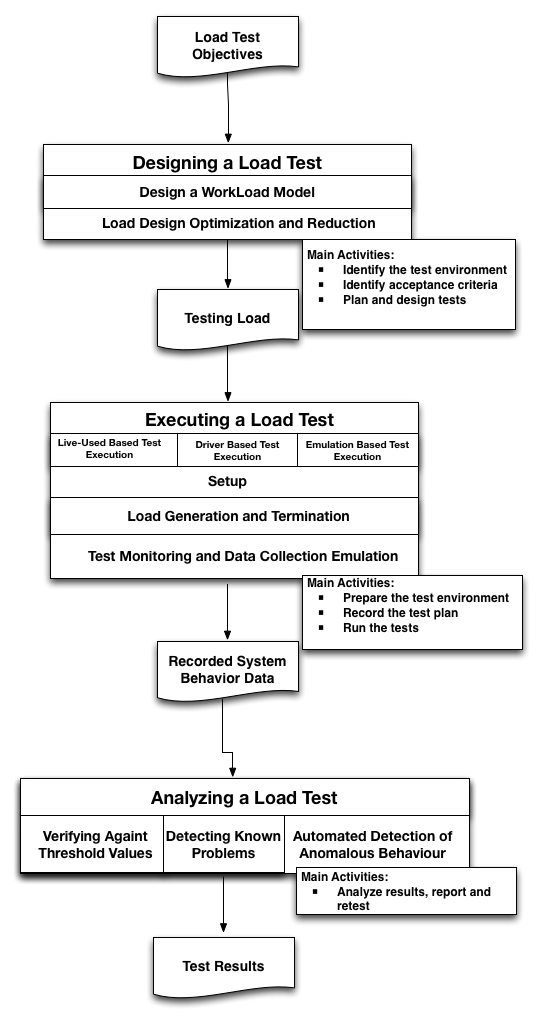
\includegraphics[width=0.5\textwidth]{./images/testprocess.png}
\caption{Load, Performance and Stress Test Process \cite{Jiang2010}\cite{Erinle2013}}
\label{fig:testprocess}
\end{figure}


The goal of the load design phase is to devise a load, which can uncover non-functional problems. Once the load is defined, the system under test executes the load and the system behavior under load is recorded. Load testing practitioners then analyze the system behavior to detect problems \cite{Jiang2010}. 

Once a proper load is designed, a load test is executed. The load test execution phase consists of the following three main aspects: (1) Setup, which includes system deployment and test execution setup; (2) Load Generation and Termination, which consists of generating the load; and (3) Test Monitoring and Data Collection, which includes recording the system behavior during execution\cite{Jiang2010}. 

The core activities in conducting an usual Load, Performance and Stress tests are \cite{Erinle2013}: 

\begin{itemize}
\item Identify the test environment: identify test and production environments and knowing the hardware, software, and network configurations helps derive an effective test plan and identify testing challenges from the outset.

\item Identify acceptance criteria: identify the response time, throughput, and resource utilization goals and constraints.

\item Plan and design tests:identify the test scenarios.In the context of testing, a scenario is a sequence of steps in an application. It can represent a use case or a business function such as searching a product catalog, adding an item to a shopping cart, or placing an order \cite{Corporation2007}.

\item Prepare the test environment: configure the test environment, tools, and resources necessary to conduct the planned test scenarios.

\item Record the test plan: record the planned test scenarios using a testing tool.

\item Run the tests: Once recorded, execute the test plans under light load and verify the correctness of the test scripts and output results.

\item Analyze results, report, and retest: examine the results of each successive run and identify areas of bottleneck that need addressing.  

\end{itemize}



\subsection{Automated Stress Test Tools}

Automated tools are needed to carry out serious load, stress, and performance testing. Sometimes, there is simply no practical way to provide reliable, repeatable performance tests without using some form of automation. The aim of any automated test tool is to simplify the testing process. Automated Test Tool  typically have the following components \cite{Molyneaux2009}:

\begin{itemize}
\item Scripting module: Enable recording of end-user activities in different middleware protocols;
\item Test management module: Allows the creation of test scenarios;
\item Load injectors: Generate the load with multiple workstations or servers;
\item Analysis module: Provides the ability to analyse the data collected by each test interation.
\end{itemize}

Apache JMeter is a free open source stress testing tool.  It has a large user base and offers lots of plugins to aid testing. JMeter is a desktop application designed to test and measure the performance and functional behavior of applications. The application it's purely Java-based and is highly extensible through a provided API (Application Programming Interface). JMeter works by acting as the client of a client/server application. JMeter allows multiple concurrent users to be simulated on the application \cite{Halili2008} \cite{Erinle2013}. 

JMeter has components organized  in a hierarchical manner. The Test Plan is the main component in a JMeter script. A typical test plan will consist of one or more Thread Groups, logic controllers, listeners, timers, assertions, and configuration elements:

\begin{itemize}
\item Thread Group: Test management module responsible to simulate the users used in a test. All elements of a test plan must be under a thread group.
\item Listeners: Analysis module responsible to provide access to the information gathered by JMeter about the test cases .
\item Samplers: Load injectors module responsible to send requests to a server, while Logical Controllers let you customize its logic.
\item Timers: allow JMeter to delay between each request.
\item Assertions: test if the application under test it is returning the correct results.
\item Configuration Elements: configure detais about the request protocol and test elements.
\end{itemize}


\subsection{Stress Test Results}

The system behavior recorded during the test execution phase needs to be analyzed to determine if there are any load-related functional or non-functional problems \cite{Jiang2010}.

There can be many formats of system behavior like resource usage data or end-to-end response time, which is recorded as response time for each individual request. These types of data need to be processed before comparing against threshold values.A proper data summarization technique is needed to describe these many data instances into one number. Some researchers advocate that the 90-percentile response time is a better measurement than the average/medium response time, as the former accounts for most of the peaks, while eliminating the outliers \cite{Jiang2010}.




\section{WorkLoad Model}

Load, performance, or stress testing projects should start with the development of a model for user workload that an application receives. This should take into consideration various performance aspects of the application and the infrastructure that a given workload will impact. A workload is a key component of such a model \cite{Molyneaux2009}.

The term workload represents the size of the demand that will be imposed on the application under test in an execution. The metric  used for measure a workload is dependent on the application domain, such as the length of the video in a transcoding application for multimedia files or the size of the input files in a file compression application \cite{Feitelson2013} \cite{Molyneaux2009} \cite{Goncalves2014}. 

Workload is also defined by the load distribution between the identified transactions at a given time. Workload helps researchers study the system behavior identified in several load models. A workload model can be designed to verify the predictability, repeatability, and scalability of a system \cite{Feitelson2013} \cite{Molyneaux2009}.


Workload modeling is the attempt to create a simple and generic model that can then be used to generate synthetic workloads. The goal is typically to be able to create workloads that can be used in performance evaluation studies. Sometimes, the synthetic workload is supposed to be similar to those that occur in practice in real systems \cite{Feitelson2013} \cite{Molyneaux2009}.

There are two kinds of workload models: descriptive and generative. The main difference between the two is that descriptive models just try to mimic the phenomena observed in the workload, whereas generative models try to emulate the process that generated the workload in the first place \cite{DiLucca2006}. 

In descriptive models, one finds different levels of abstraction on the one hand and different levels of fidelity to the original data on the other hand. The most strictly faithful models try to mimic the data directly using the statistical distribution of the data. The most common strategy used in descriptive modeling is to create a statistical model of an observed workload (Fig. \ref{fig:descriptivemodel}). This model is applied to all the workload attributes, e.g., computation, memory usage, I/O behavior, communication, etc. \cite{DiLucca2006}. Fig. \ref{fig:descriptivemodel} shows a simplified workflow of a descriptive model. The workflow has six phases. In the first phase, the user uses the system in the production environment. In the second phase, the tester collects the user's data, such as logs, clicks, and preferences, from the system. The third phase consists in developing a model designed to emulate the user's behavior. The fourth phase is made up of the execution of the test, emulation of the user's behavior, and log gathering.



\begin{figure}[!ht]
\begin{minipage}{.5\textwidth}
\centering
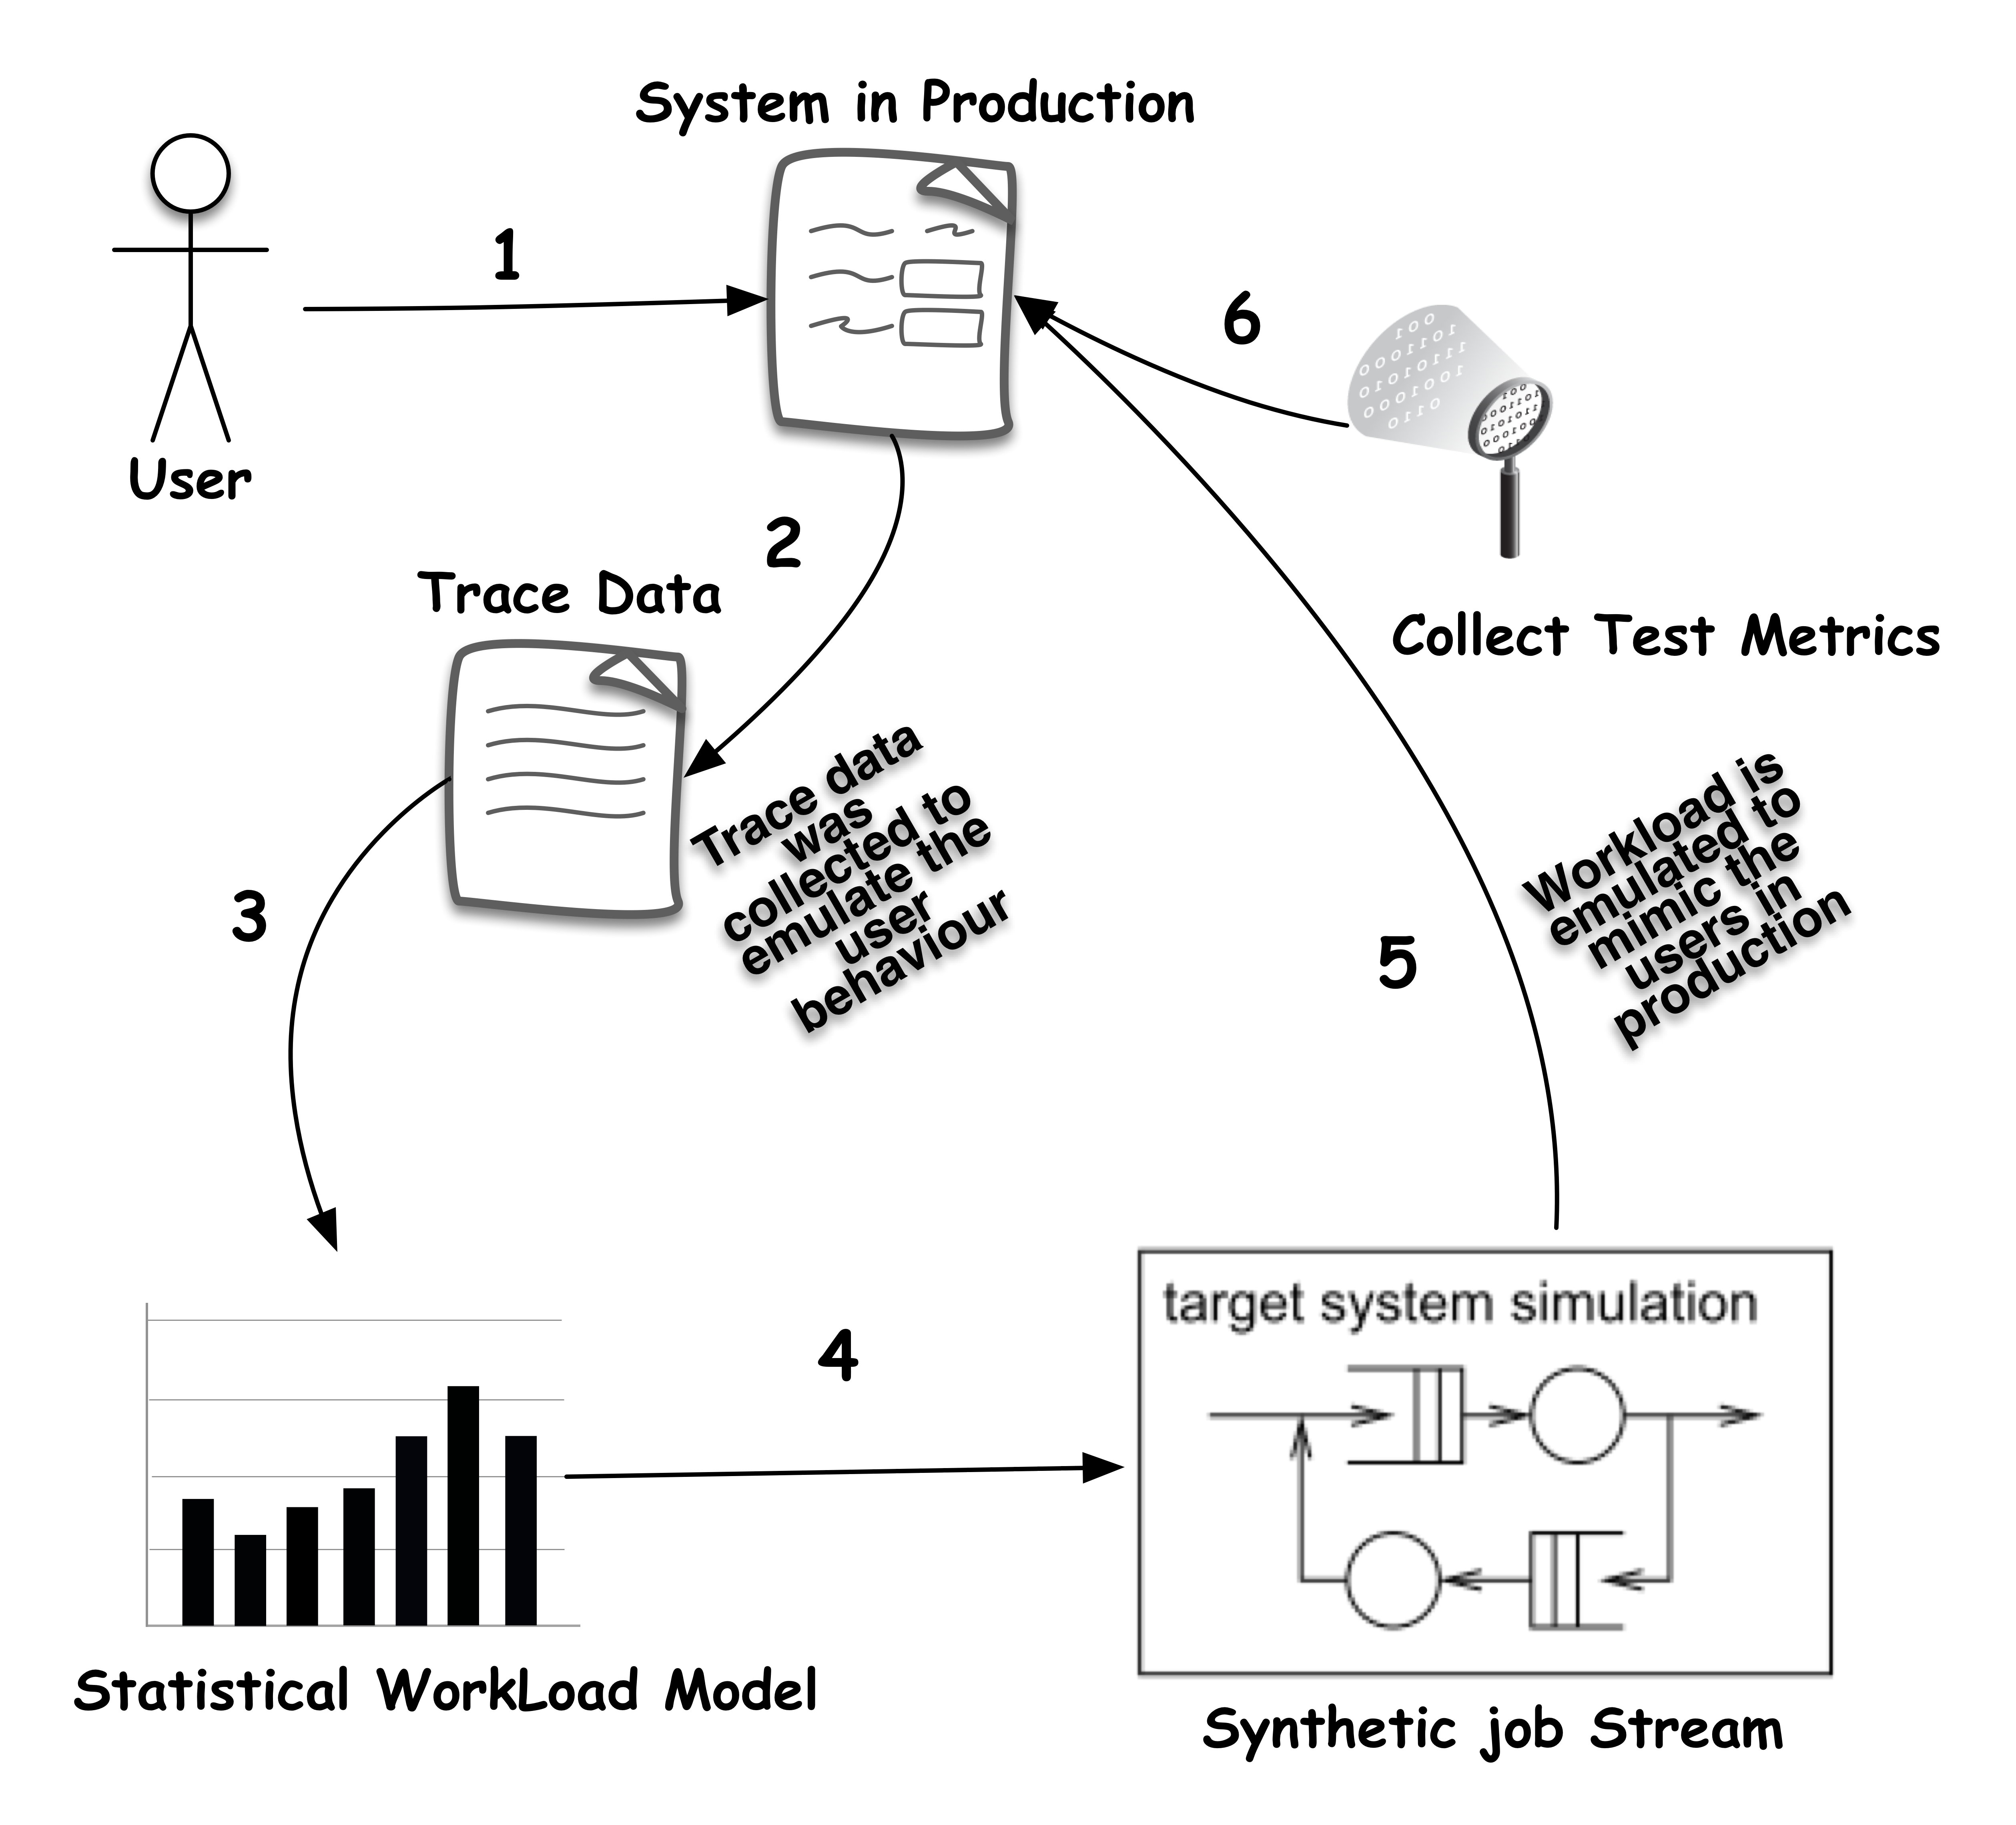
\includegraphics[width=0.8\textwidth]{./images/workloadmodel1300dpi.png}
\caption{Workload modeling based on statistical data \cite{DiLucca2006}}
\label{fig:descriptivemodel}
\end{minipage}
\begin{minipage}{.5\textwidth}
\centering
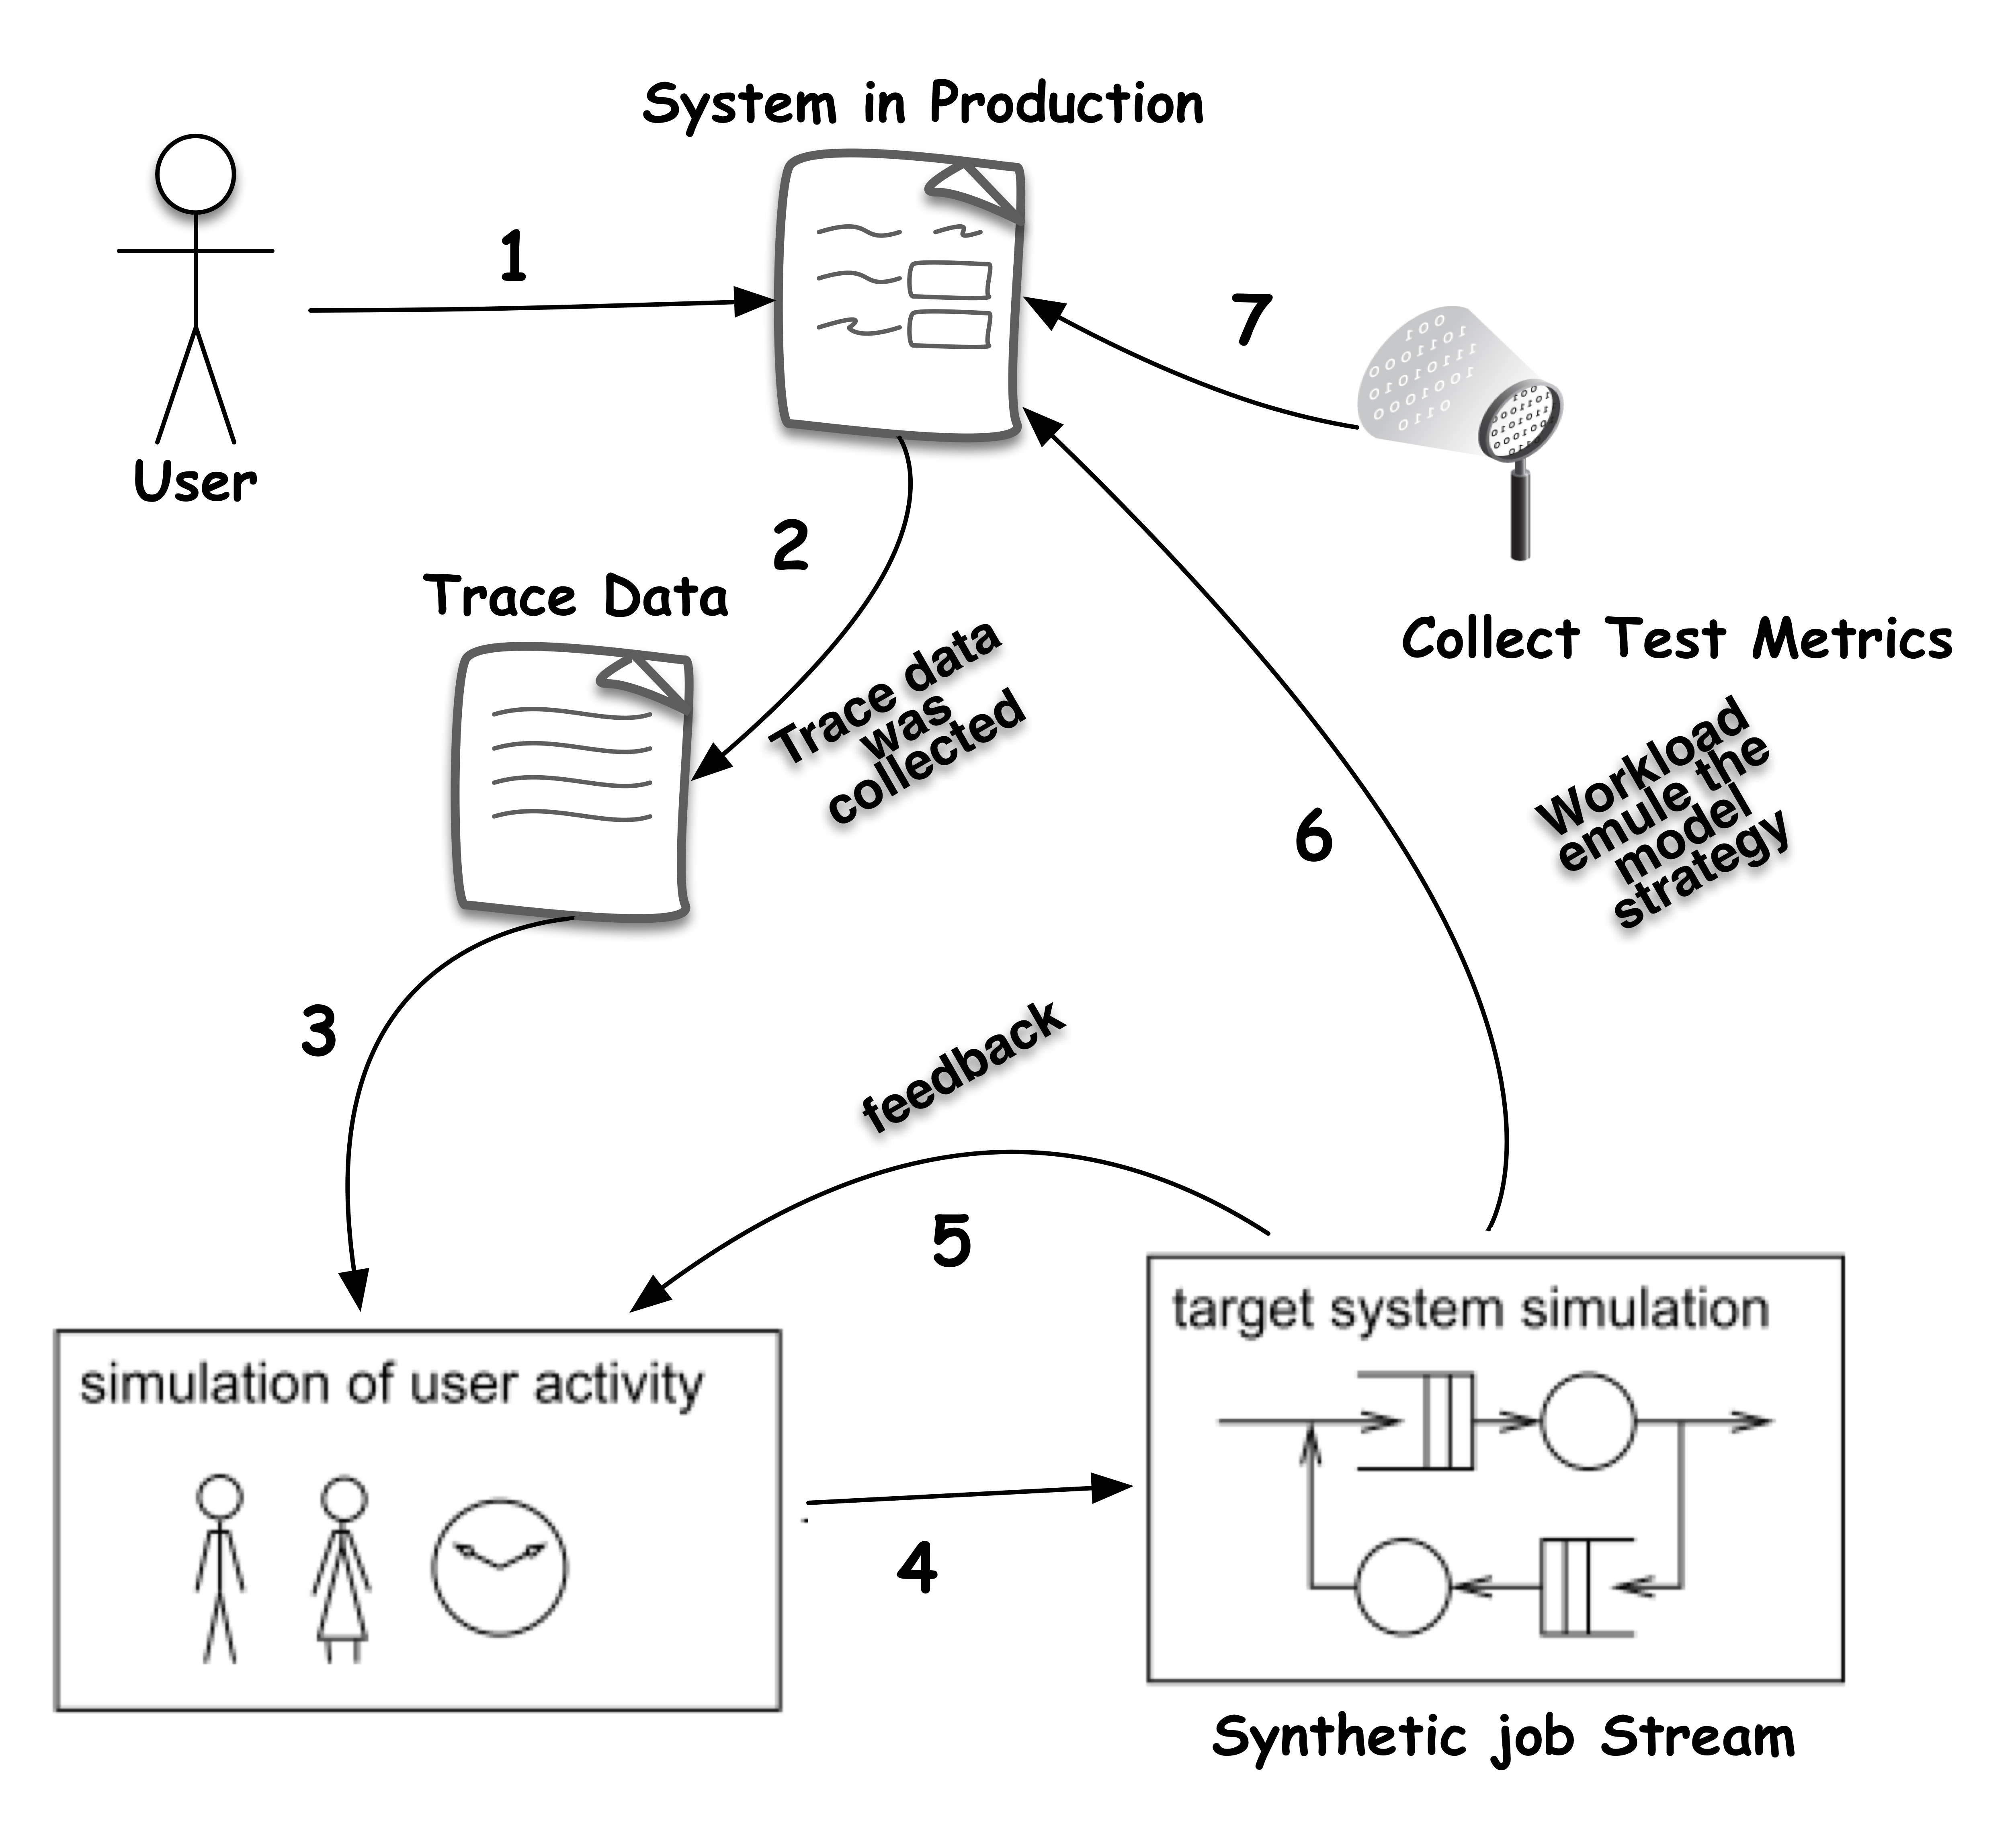
\includegraphics[width=0.8\textwidth]{./images/workloadmodel2300dpi.png}
\caption{Workload modeling based on the generative model \cite{DiLucca2006}}
\label{fig:generativemodel}
\end{minipage}
\end{figure}

Generative models are indirect in the sense that they do not model the statistical distributions. Instead, they describe how users will behave when they generate the workload. An important benefit of the generative approach is that it facilitates manipulations of the workload. It is often desirable to be able to change the workload conditions as part of the evaluation. Descriptive models do not offer any option regarding how to do so. With the generative models, however, we can modify the workload-generation process to fit the desired conditions \cite{DiLucca2006}. The difference between the workflows of the descriptive and the generative models is that user behavior is not collected from logs, but simulated from a model that can receive feedback from the test execution (Fig. \ref{fig:generativemodel}).

Both load model have their advantages and disadvantages. In general, loads resulting from realistic-load based design techniques (Descriptive models) can be used to detect both functional and non-functional problems. However, the test durations are usually longer and the test analysis is more difficult. Loads resulting from fault-inducing load design techniques (Generative models) take less time to uncover potential functional and non-functional problems, the resulting loads usually only cover a small portion of the testing objectives \cite{Jiang2010}. The presented research work uses a generative model.



\section{Common performance application problems and performance antipatterns}

Performance is critical to the success of today’s software systems. Many software products fail to meet their performance objectives when they are initially constructed. Performance problems share common symptoms and many performance problems described in the literature are defined by a particular set of root causes. Fig. \ref{fig:symptoms}  shows the symptoms of known performance problems \cite{Wert2013a}. 



\begin{figure}[h]
\centering
\includegraphics[width=0.5\textwidth]{./images/symptoms.png}
\caption{Symptoms of know performance problems \cite{Wert2013a}. }
\label{fig:symptoms}
\end{figure}


There are several antipatterns that details features about  common performance problems. Antipatterns are conceptually similar to patterns in that they document recurring solutions to common design problems. They are known as
antipatterns because their use produces negative consequences.  Performance antipatterns document common performance mistakes made in software architectures or designs. These software Performance antipatterns have four primary uses: identifying problems,
focusing on the
right level of abstraction,
effectively communicating
their causes to others, and prescribing solutions \cite{brown1998antipatterns}. The table \ref{antipatterns} present some of the most common performance antipatterns.


% Please add the following required packages to your document preamble:
% \usepackage{multirow}
% \usepackage[table,xcdraw]{xcolor}
% If you use beamer only pass "xcolor=table" option, i.e. \documentclass[xcolor=table]{beamer}
\begin{table}[H]
\centering
\caption{Performance antipatterns}
\label{antipatterns}
\begin{tabular}{|l|l|}
\hline
\rowcolor[HTML]{C0C0C0} 
\multicolumn{1}{|c|}{\cellcolor[HTML]{C0C0C0}\textbf{antipattern}} & \multicolumn{1}{c|}{\cellcolor[HTML]{C0C0C0}\textbf{Derivations}} \\ \hline
Blob or The God Class &  \\ \hline
 & Concurrent processing Systems \\ \cline{2-2} 
 & Piper and Filter Architectures \\ \cline{2-2} 
\multirow{-3}{*}{Unbalanced-Processing} & Extensive Processing \\ \hline
Circuitous Treasure Hunt &  \\ \cline{1-1}
Empty Semi Trucks &  \\ \cline{1-1}
Tower of Babel &  \\ \cline{1-1}
One-Lane Bridge &  \\ \cline{1-1}
Excessive Dynamic Allocation &  \\ \cline{1-1}
Traffic Jam &  \\ \cline{1-1}
The Ramp  &  \\ \cline{1-1}
More is Less & \multirow{-10}{*}{} \\ \hline
\end{tabular}
\end{table}

Blob antipattern is known by various names, including the “god” class [8] and the “blob” [2]. Blob is an antipattern whose problem is on the excessive message traffic generated by a single class or component, a particular resource does the majority of the work in a software. The Blob antipattern occurs when a single class or component either performs all of the work of an application or holds all of the application’s data. Either manifestation results in excessive message traffic that can degrade performance \cite{Cortellessa2007} \cite{Smith2000}.

A project containing a “god” class is usually has a single, complex controller class that is surrounded by simple classes that serve only as data containers. These classes typically contain only accessor operations (operations to get() and set() the data) and perform little or no computation of their own \cite{Smith2000}.
The  Figures \ref{fig:godclass} and \ref{fig:godclass2} describes an hypotetical system with a BLOB problem:
The Fig. \ref{fig:godclass} presents a sample where the Blob class uses the features A,B,C,D,E,F and G of the hypotetical system; The Fig. \ref{fig:godclass2}  shows a static view where  a complex software entity instance, i.e. Sd, is connected to other software instances, e.g. Sa, Sb and Sc, through many dependencies \cite{Vetoio2011}\cite{Wert2013a}.




\begin{figure}[h]
\begin{minipage}{.5\textwidth}
\centering
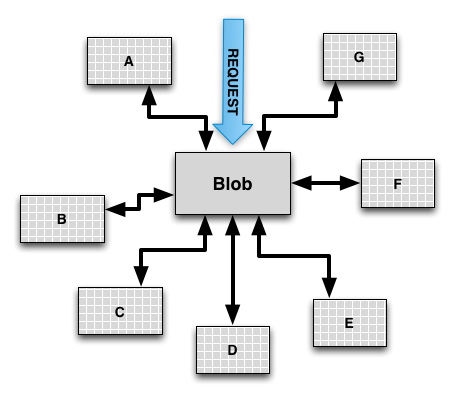
\includegraphics[width=1\textwidth]{./images/BLOB.png}
\caption{The God class\cite{Wert2013a}. }
\label{fig:godclass}
\end{minipage}
\begin{minipage}{.5\textwidth}
\centering
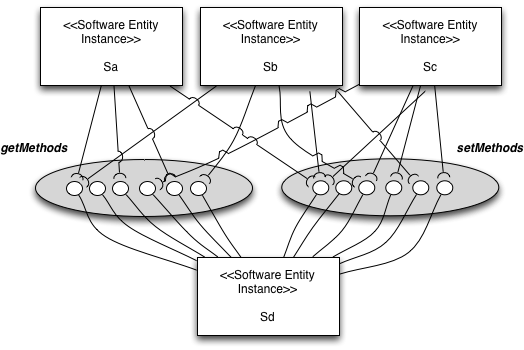
\includegraphics[width=1\textwidth]{./images/blob2.png}
\caption{The God class\cite{Vetoio2011}. }
\label{fig:godclass2}
\end{minipage}
\end{figure}

Unbalanced Processing it's characterizes for one scenario where a specific class of requests generates a pattern of execution within the system that tends to overload a particular resource. In other words the overloaded resource will be executing a certain type of job very often, thus in practice damaging other classes
of jobs that will experience very long waiting times. Unbalanced Processing occurs in three different situations. The first case that cause unbalanced processing it is when processes cannot make effective use of available processors either because processors are dedicated to other tasks or because of single-threaded code. This manifestation has available processors and we need to ensure that the software is able to use them. Fig. \ref{fig:unbalanced}  shows a sample of the Unbalanced Processing. In The Fig. \ref{fig:unbalanced}, four tasks are performed. The task D it is waiting for the task C conclusion that are submmited to a heavy processing situation. 

The pipe and filter architectures  and extensive processing antipattern represents a manifestation of the unbalanced processing antipattern. The pipe and filter architectures occurs when the throughput of the overall system is determined by the slowest filter. The  Fig. \ref{fig:pipefilter} describes a software S with a Pipe and Filter Architectures problem: (a) Static View, there is a software entity instance, e.g. Sa, offering an operation (operation x) whose resource demand (computation = \$compOpx, storage = \$storOpx, bandwidth = \$bandOpx) is quite high; (b) Dynamic View, the operation opx is invoked in a service  and the throughput of the service (\$Th(S)) is lower than the required one. The extensive processing occurs when a process monopolizes a processor and prevents a set of other jobs to be executed until it finishes its computation. The Fig. \ref{fig:extpro} describes a software S with a Extensive Processing problem: (a) Static View, there is a software entity instance, e.g. Sa, offering two operations (operation x, operation y) whose resource demand is quite unbalanced, since opx has a high demand (computation = \$compOpx, storage = \$storOpx, bandwidth = \$bandOpx), whereas opy has a low demand (computation = \$compOpy, storage = \$storOpy, bandwidth = \$bandOpy); (b) Dynamic View, the operations opx and opy are alternatively invoked in a service and the response time of the service (\$RT(S)) is larger than the required one \cite{Vetoio2011}.

\begin{figure}[h]
\centering
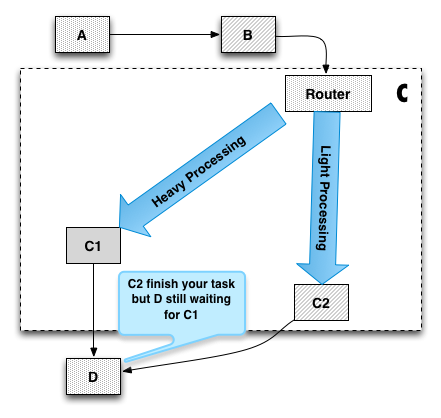
\includegraphics[width=0.5\textwidth]{./images/unbalanced.png}
\caption{Unbalanced Processing sample \cite{Wert2013a}. }
\label{fig:unbalanced}
\end{figure}


\begin{figure}[h]
\begin{minipage}{.5\textwidth}
\centering
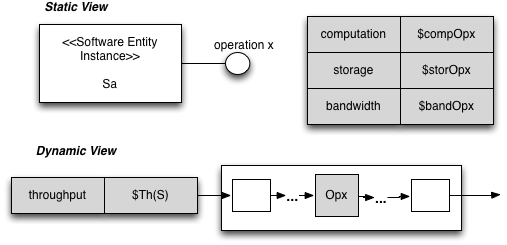
\includegraphics[width=1\textwidth]{./images/pipe2.png}
\caption{Pipe and Filter sample \cite{Vetoio2011}}
\label{fig:pipefilter}
\end{minipage}
\begin{minipage}{.5\textwidth}
\centering
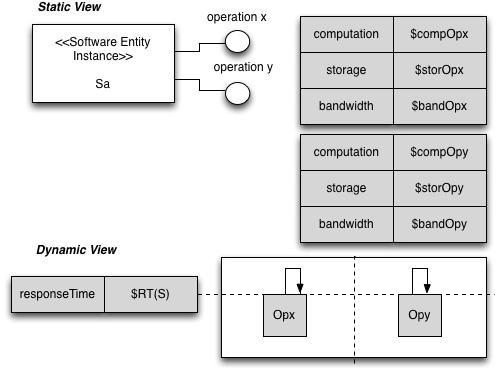
\includegraphics[width=1\textwidth]{./images/extpro.png}
\caption{Extensive Processing sample \cite{Vetoio2011}.}
\label{fig:extpro}
\end{minipage}
\end{figure}


Circuitous Treasure Hunt antipattern occurs when software retrieves data from a first componet, uses those results in a second component, retrieves data from the second component, and so on, until the last results are obtained \cite{Smith2002} \cite{Smith2003}. Circuitous Treasure Hunt 
are typical performance antipatterns that causes unnecessarily frequent database requests. The Circuitous Treasure Hunt antipattern is a result from a bad database schema or query design. A common Circuitous Treasure Hunt design creates a data dependency between single queries. For instance, a query requires the
result of a previous query as input. The longer the chain of
dependencies between individual queries the more the Circuitous
Treasure Hunt antipattern hurts performance \cite{Wert2014}. The Fig. \ref{fig:circuit}  shows a software S with a Circuitous Treasure Hunt problem: (a) Static View, there is a software entity instance e.g. Sa, retrieving information from the database; (b) Dynamic View, the software  S generates a large number of database calls by performing several queries up to the final operation \cite{Vetoio2011}.


\begin{figure}[h]
\begin{minipage}{.5\textwidth}
\centering
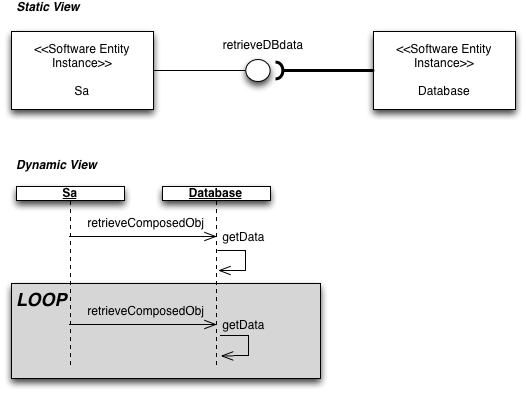
\includegraphics[width=1\textwidth]{./images/circuit.png}
\caption{Circuitous
Treasure Hunt sample \cite{Vetoio2011}}
\label{fig:circuit}
\end{minipage}
\begin{minipage}{.5\textwidth}
\centering
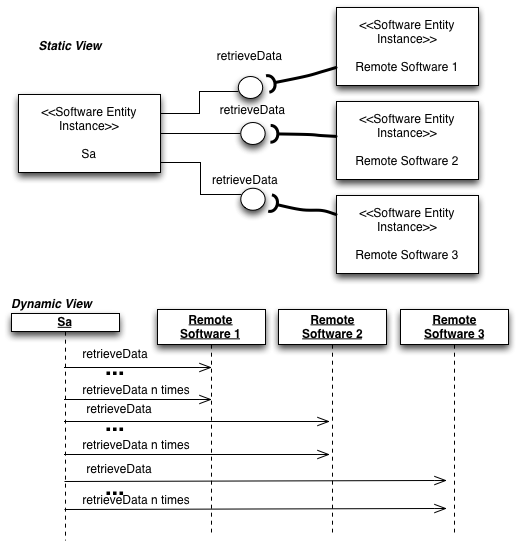
\includegraphics[width=1\textwidth]{./images/trucks.png}
\caption{Empty Semi Trucks sample \cite{Vetoio2011}.}
\label{fig:trucks}
\end{minipage}
\end{figure}

Empty Semi Trucks occurs when an excessive number of requests is required to perform a task. It may be due to inefficient use of available bandwidth, an inefficient interface, or both \cite{Arcelli2012}. There are a special case of Empty Semi Trucks that occurs  when many fields in a user interface must be retrieved from a
remote system. Fig. shows a software S with a Empty Semi Trucks problem: (a) Static View, there is a software entity instance, e.g. Sa, retrieving some information from several instances (Remote Software 1, . . . , Remote Software n); (b) Dynamic View, the software instance Sa generates an excessive message traffic by sending a big amount of messages with low sizes, much lower than the network bandwidth, hence the network link might have a low utilization value \cite{Vetoio2011}.

The Tower of Babel antipattern most often occurs when information is translated into an exchange format, such as XML, by the sending process then parsed and translated into an
internal format by the receiving process. When the translation and parsing is excessive, the system spends most
of its time doing this and relatively little doing real work \cite{Smith2003}. Fig. shows a system with a Tower of Babel problem: (a) Static View, there are some software entity instances, e.g. Sa, Sb, . . . , Sn; (b) Dynamic View, the software instances Sd performs many times the translation of format for communicating with other instances \cite{Vetoio2011}.

\begin{figure}[h]
\begin{minipage}{.5\textwidth}
\centering
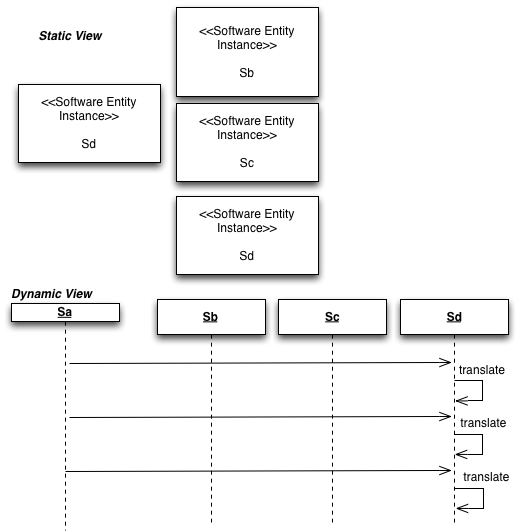
\includegraphics[width=1\textwidth]{./images/babel2.png}
\caption{Tower of Babel sample \cite{Vetoio2011}}
\label{fig:babel}
\end{minipage}
\begin{minipage}{.5\textwidth}
\centering
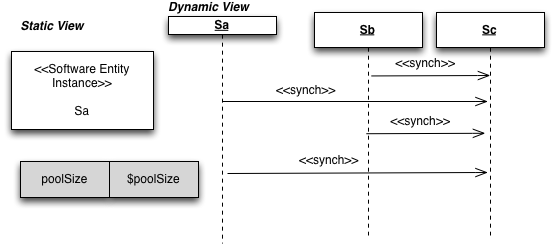
\includegraphics[width=1\textwidth]{./images/onelane.png}
\caption{One-Lane Bridge sample \cite{Vetoio2011}.}
\label{fig:onelane}
\end{minipage}
\end{figure}


One-Lane Bridge is a antipattern that occurs when one or a few processes execute concurrently using a shared resource and other processes are waiting for use the shared resource. It frequently occurs in applications that access a database. Here, a lock ensures that only one process may update the associated portion of the database at a time. This antipatterns is common when many concurrent threads or processes are waiting for the same shared resources. These can either be passive resources (like semaphores or mutexes) or active resources (like CPU or hard disk). In the first case, we have a typical One Lane Bridge whose critical resource needs to be identified. Figure 3.10 shows a system with a One-Lane Bridge problem: (a) Static View, there is a software entity instance with a capacity of managing \$poolSize threads; (b) Dynamic View, the software instance Sc receives an excessive number of synchronous calls in a service S and the predicted response time is higher than the required \cite{Vetoio2011}.


Using dynamic allocation, objects are created when they are first accessed and then destroyed when they are no longer needed. Excessive Dynamic Allocation, however, addresses frequent, unnecessary creation and destruction of objects of the same class. Dynamic allocation is expensive , an object created in memory must be allocated from the heap, and any initialization code for the object and the contained objects must be executed. When the object is no longer needed, necessary clean-up must be performed, and the reclaimed memory must be returned to the heap to avoid memory leaks \cite{Smith2002} \cite{Smith2003}.

\begin{figure}[h]
\begin{minipage}{.5\textwidth}
\centering
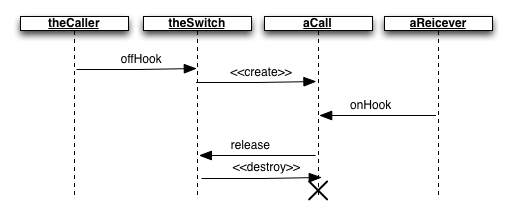
\includegraphics[width=1\textwidth]{./images/excessivedynamicallocation.png}
\caption{Excessive Dynamic Allocation.}
\label{fig:dynallocation}
\end{minipage}
\begin{minipage}{.5\textwidth}
\centering
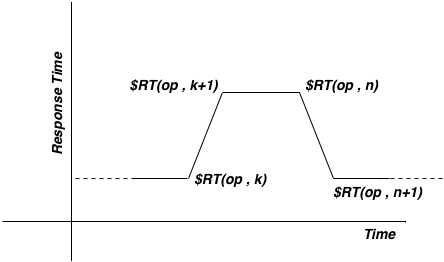
\includegraphics[width=1\textwidth]{./images/jam.png}
\caption{Traffic Jam Response Time \cite{Vetoio2011}.}
\label{fig:jam}
\end{minipage}
\end{figure}

The Fig. \ref{fig:dynallocation} shows a Excessive Dynamic Allocation sample. This example is drawn from a call (an offHook event), the switch creates a Call object to manage the call. When the call is completed, the Call object is destroyed. Constructing a single Call object it is not seem as excessive. A Call is a complex object that contains several other objects that must also be created. The Excessive Dynamic Allocation occurs when  a switch receive hundreds of thousands of offHook events. In a case like this, the overhead for dynamically allocating call objects adds substantial delays to the time needed to complete a call.

The Traffic Jam antipattern occurs if many concurrent threads or processes are waiting for the same  active resources (like CPU or hard disk). This antipatterns produces a large backlog in jobs waiting for service. The performance impact of the Traffic Jam is the transient behavior that produces wide variability in response time. Sometimes it is fine, but at other times, it is unacceptably long. Figure \ref{fig:jam} describes a software with a Traffic Jam problem, the monitored response time of the operation shows a wide variability in response time which persists long \cite{Vetoio2011}. 


\begin{figure}[h]
\begin{minipage}{.5\textwidth}
\centering
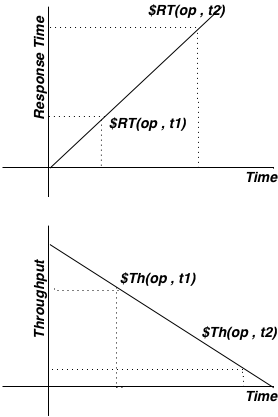
\includegraphics[width=0.5\textwidth]{./images/ramp.png}
\caption{The Ramp sample \cite{Vetoio2011}.}
\label{fig:ramp}
\end{minipage}
\begin{minipage}{.5\textwidth}
\centering
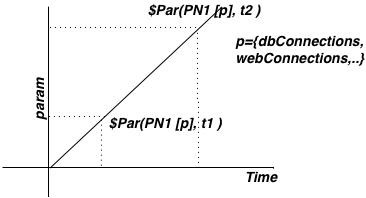
\includegraphics[width=1\textwidth]{./images/moreisless.png}
\caption{More is Less sample \cite{Vetoio2011}.}
\label{fig:moreisless}
\end{minipage}
\end{figure}

The Ramp it is a antipattern where the processing time increases as the system is used. The Ramp can arise in several different ways. Any situation in which the amount of processing required to satisfy a request increases over time will produce the behavior. With the Ramp antipattern, the memory consumption of the application is growing over time. The root cause is Specific Data Structures which are growing during operation or which are not properly disposed \cite{Wert2014} \cite{Smith2003}. Fig. \ref{fig:ramp} shows a system  with The Ramp problem:  (i) the monitored response time of the operation opx at time t1, i.e. \$RT(opx, t1), is much lower than the monitored response time of the operation opx at time t2, i.e. \$RT(opx, t2), with t1 < t2; (ii) the monitored throughput of the operation opx at time t1, i.e. \$Th(opx, t1), is much larger than the monitored throughput of the operation opx at time t2, i.e. \$Th(opx, t2), with t1 < t2. 

More is less occurs when a system spends more time "thrashing” than accomplishing real work because there are too many processes relative to available resources. More is Less are presented when it is running too many programs overtime. This antipattern causes too much system paging and systems spend all their time servicing page faults rather than processing requests. In distributed systems, there are more causes.They include: creating too many database connections and  allowing too many internet connection. Fig. \ref{fig:moreisless} describes a system  with a More Is Less problem: There is a processing node PN1 and the monitored runtime parameters (e.g. database connections, etc.) at time t1, i.e. \$Par(PN1[p], t1), are much larger than the same parameters at time t2, i.e. \$Par(PN1[p], t2), with t1 < t2. 


To emulate the presented antipatterns the testbed solution uses Mock Objects with the JMeter load test tool.

\section{Mock Objects}

A Mock Object is a substitute implementation to emulate other domain code. It
should be simpler than the real code, not duplicate its implementation \cite{Mackinnon2001}. There are several reasons to use Mock Objects \cite{Hunt2002}:

\begin{itemize}
\item The real object has nondeterministic
behavior.
\item The real object is difficult to set up.
\item The real object has behavior that is hard to trigger (for example, a network error).
\item The real object is slow.
\item The real object has (or is) a user
interface.
\item The test needs to ask the real object
about how it was used (for example,
a test might need to check
to see that a callback function was
actually called).
\item The real object does not yet exist.
\end{itemize}

\section{Search Based Tests}

Search-based software engineering (SBSE) is the application of optimization techniques in solving software engineering problems [1,2]. The applicability of optimization techniques in solving software engineering problems is suitable as these problems frequently encounter competing constraints and require near optimal solutions \cite{Afzal2009a} \cite{Harman2015}. 


Search Based Software Testing (SBST) is the sub-area of Search Based Software Engineering concerned with software testing. Search-based software testing is the application of metaheuristic search techniques to generate software tests. SBSE uses computational search techniques to tackle software engineering problems, typified by large complex search spaces. SBSE derives test inputs for a software system with the goal of improving various criteria. The test adequacy criterion is transformed into a fitness function and a set of solutions in the search space are evaluated with respect to the fitness function using a metaheuristic search technique \cite{Afzal2009a} \cite{Aleti2016} \cite{Harman2015}.

Figure \ref{fig:sbsesbst}  shows the growth in papers published on SBST and SBSE. The data is taken from the SBSE repository (\url{http://crestweb.cs.ucl.ac.uk/resources/sbse_repository/}). 
The aim of the SBSE repository is to contain every SBSE paper. Although no repository can guarantee 100\% precision and recall, the SBSE repository has proved sufficiently usable that it has formed the basis of several other detailed analyses of the literature \cite{Harman2015}. 


\begin{figure}[h]
\begin{minipage}{.5\textwidth}
\centering
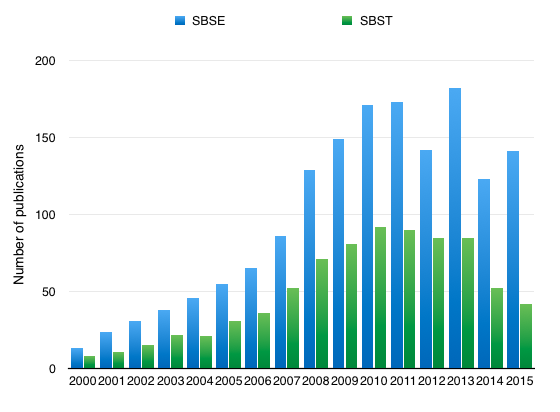
\includegraphics[width=0.8\textwidth]{./images/publications1.png}
\caption{Number of publications in SBSE and SBST by Year. Data comes from the Harman et al., Afzal et al. and the SBSE repository  \cite{Afzal2009a} \cite{Harman2015}}
\label{fig:sbsesbst}
\end{minipage}
\begin{minipage}{.5\textwidth}
\centering
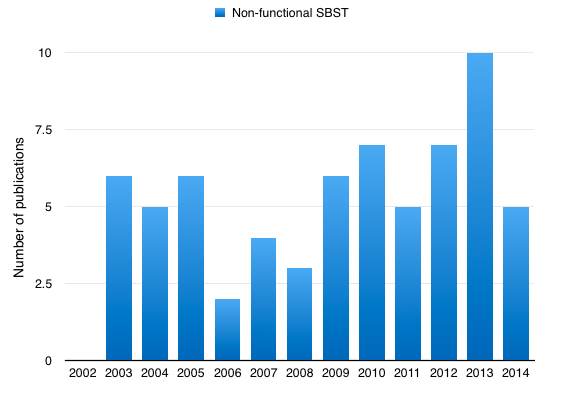
\includegraphics[width=0.8\textwidth]{./images/nonfunctional.png}
\caption{Number of publications in non-functional SBST by Year. Data comes from the Harman et al., Afzal et al. and the SBSE repository  \cite{Afzal2009a} \cite{Harman2015} }
\label{fig:nonfunctional}
\end{minipage}
\end{figure}


SBST has made many achievements, and demonstrated its wide applicability and increasing uptake. Nevertheless, there are pressing open problems and challenges that need more attention like to extend SBST to test non-functional properties, a topic that remains relatively under-explored, compared to structural testing. The Fig. \ref{fig:nonfunctional} shows the non-funtional SBST by year \cite{Aleti2016} \cite{Harman2015}. 

There are many kinds of non-functional search based tests  \cite{Afzal2009a}:

\begin{itemize}
\item Execution time: The application of evolutionary algorithms to find the best and worst case execution times (BCET, WCET).
\item Quality of service: uses metaheuristic search techniques to search violations of service level agreements (SLAs).
\item Security: apply a variety of metaheuristic search techniques  to detect security vulnerabilities like detecting buffer overflows.
\item Usability: concerned with construction of covering array which is a combinatorial object.
\item Safety: Safety testing is an important component of the testing strategy of safety critical systems where the systems are required to meet safety constraints.
\end{itemize}

A variety of metaheuristic search techniques are found to be applicable for non-functional testing including simulated annealing, tabu search, genetic algorithms, ant colony methods, grammatical evolution, genetic programming and swarm intelligence methods. The Fig. \ref{fig:metabykind} shows a comparison between the range of metaheuristcs and the type of non-functional search based test.The Data comes from Afzal et al. \cite{Afzal2009}. Afzal's work adds to some of the latest research in this area (\cite{Garousi2006} \cite{Garousi2010} \cite{DiAlesio2013} \cite{DiAlesio2014} \cite{Alesio2015} \cite{Gois2016}). 


\begin{figure}[h]
\centering
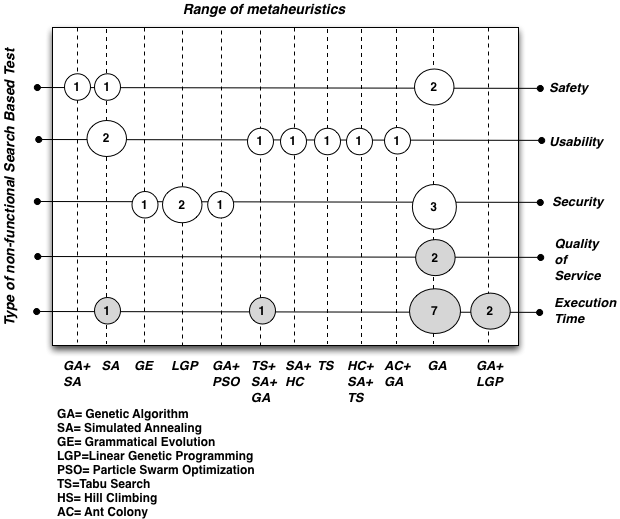
\includegraphics[width=0.6\textwidth]{./images/metaheuristics.png}
\caption{Range of metaheuristics by Type of non-functional Search Based Test\cite{Afzal2009a}. }
\label{fig:metabykind}
\end{figure}

\subsection{Load, Stress and Performance Search Based Testing}

A common goal of load, performance and stress search-based testing is to find test scenarios that produce execution times that exceed the timing constraints specified. If a temporal error is found, the test was successful \cite{Sullivan}. The search for the longest execution time is regarded as a discontinuous, nonlinear, optimization problem, with the input domain of the system under test as a search space \cite{Sullivan}.  The application of SBST algorithms to  stress tests involves finding the best- and worst-case execution times (B/WCET) to determine whether timing constraints are fulfilled \cite{Afzal2009a}. 

There are two measurement units normally associated with the fitness function in stress test: processor cycles and execution time. The processor cycle approach describes a fitness function in terms of processor cycles. The execution time approach involves executing the application under test and measuring the execution time \cite{Afzal2009a} \cite{tracey2000search}.

Processor cycles measurement is deterministic in the sense that it is independent of system load and results in the same execution times for the same set of input parameters. However, such a measurement is dependent on the compiler and optimizer used, therefore, the processor cycles differ for each platform. Execution time measurement is a non deterministic approach, there is no guarantee to get the same results for the same test inputs \cite{Afzal2009a}.  However, stress testing where testers have no access to the production environment should be measured by the execution time measurement \cite{Molyneaux2009} \cite{Afzal2009a}.

Table \ref{tab:comparison}  shows a comparison between the research studies on load, performance, and stress tests presented by Afzal et al. \cite{Afzal2009}. Afzal's work adds to some of the latest research in this area (\cite{Garousi2006} \cite{Garousi2010} \cite{DiAlesio2013} \cite{DiAlesio2014} \cite{Alesio2015} \cite{Gois2016} ). The columns represent the type of tool used (prototype or functional tool), and the rows represent the metaheuristic approach used by each research study (genetic algorithm, Tabu search, simulated annealing, or a customized algorithm). The table also sorts the research studies by the type of fitness function used (execution time or processor cycles). 

\begin{table}[h]
\centering
\caption{Distribution of the research studies over the range of applied metaheuristics}
\label{tab:comparison}
\begin{tabular}{p{1.2cm}|p{1.8cm}|p{1.8cm}|p{1.8cm}|}
\cline{2-4}
                                                                & \multicolumn{2}{c|}{\textbf{Prototypes}}            & \textbf{Functional Tool} \\ \cline{2-4} 
                                                                & \begin{minipage}{0.2\textwidth}\footnotesize Execution Time  \end{minipage}          & \begin{minipage}{0.2\textwidth}\footnotesize Processor Cycles \end{minipage}        & \begin{minipage}{0.2\textwidth}\footnotesize Execution Time \end{minipage}           \\ \cline{2-4} 
%\setlength{\extrarowheight}{20pt}
\begin{tabular}[c]{@{}l@{}}\begin{minipage}{0.1\textwidth}\scriptsize GA + SA  \\ + Tabu \\ Search \end{minipage}\end{tabular}  & \cellcolor[HTML]{FFFFFF} & \cellcolor[HTML]{FFFFFF} & \cellcolor[HTML]{FFFFFF} \begin{minipage}{0.2\textwidth} \tiny    Gois et al. 2016 \cite{Gois2016}  \end{minipage}  \\[2ex] \cline{2-4} 
\begin{minipage}{0.1\textwidth}\scriptsize GA \end{minipage}                                                              & \cellcolor[HTML]{FFFFFF} \begin{minipage}{0.12\textwidth}   \tiny \textnormal{ \\  Alander et al.,1998 \cite{Alander} \\ Wegener et al., 1996 and 1997 \cite{Wegener1997}\cite{J.WegenerK.GrimmM.GrochtmannH.Sthamer1996} \\  Sullivan et al., 1998 \cite{Sullivan} \\ Briand et al., 2005 \cite{Briand2005} \\ Canfora et al., 2005 \cite{Canfora}  \\ }\end{minipage} & \cellcolor[HTML]{FFFFFF} \begin{minipage}{0.12\textwidth} \tiny \textrm{  \\ Wegener and Grochtmann, 1998 \cite{Wegener1998} \\  Mueller et al., 1998 \cite{Mueller1998} \\ Puschner et al. \cite{Puschner1998} \\ Wegener et al., 2000 \cite{Stations} \\ Gro et al., 2000 \cite{Gross2000}  \\ }\end{minipage}& \cellcolor[HTML]{FFFFFF} \begin{minipage}{0.12\textwidth}   \tiny \textnormal{ \\  Di Penta, 2007 \cite{Penta2007} \\ Garoussi, 2006 \cite{Garousi2006} \\ Garousi, 2008 \cite{Garousi2008} \\ Garousi, 2010 \cite{Garousi2010} \\ } \end{minipage} \\[2ex] \cline{2-4} 
\begin{minipage}{0.1\textwidth}\scriptsize Simulated \\ Annealing \\ (SA) \end{minipage}                                                             & \cellcolor[HTML]{FFFFFF} & \cellcolor[HTML]{FFFFFF} & \cellcolor[HTML]{FFFFFF} \begin{minipage}{0.12\textwidth}   \tiny  Tracey, 1998 \cite{Tracey1998} \end{minipage} \\[2ex] \cline{2-4}
\begin{minipage}{0.1\textwidth}\scriptsize  Constraint \\ Programming \end{minipage}                                                             & \cellcolor[HTML]{FFFFFF} & \cellcolor[HTML]{FFFFFF} & \cellcolor[HTML]{FFFFFF} \begin{minipage}{0.12\textwidth}   \tiny  Alesio, 2014 \cite{DiAlesio2014} \\ Alesio, 2013 \cite{DiAlesio2013}  \end{minipage} \\[2ex] \cline{2-4} 
\begin{minipage}{0.1\textwidth}\scriptsize  GA +\\ Constraint \\ Programming \end{minipage}                                                             & \cellcolor[HTML]{FFFFFF} & \cellcolor[HTML]{FFFFFF} & \cellcolor[HTML]{FFFFFF} \begin{minipage}{0.12\textwidth}   \tiny  Alesio, 2015 \cite{Alesio2015} \end{minipage} \\[2ex] \cline{2-4} 
\setlength{\extrarowheight}{20pt}
\begin{tabular}[c]{@{}l@{}}
\begin{minipage}{0.1\textwidth}\scriptsize Customized \\ Algorithm \end{minipage}\end{tabular} & \cellcolor[HTML]{FFFFFF} & \cellcolor[HTML]{FFFFFF}  \begin{minipage}{0.12\textwidth}   \tiny  \textnormal{   \raggedleft Pohlheim, 1999 \cite{Pohlheim2005}  } \end{minipage} & \cellcolor[HTML]{FFFFFF} \\[4ex] \cline{2-4}
\end{tabular}
\end{table}


Wegener et al. \cite{Wegener1997} used genetic algorithms(GA) to search for input situations that produce very long or very short execution times. The fitness function used was the execution time of an individual measured in micro seconds \cite{Wegener1997}. 

Alander et al. \cite{Alander} performed experiments in a simulator environment to measure response time extremes of protection relay software using genetic algorithms. The fitness function used was the response time of the tested software. The results showed that GA generated more input cases with longer response times \cite{Alander}. 

Wegener and Grochtmann performed a  experimentation
to compare GA with random testing. The fitness function used was duration of execution measured in processor cycles.  The results showed that, with a large number of input parameters, GA obtained more extreme execution times with less or equal testing effort than random testing \cite{J.WegenerK.GrimmM.GrochtmannH.Sthamer1996} \cite{Wegener1998} .

Gro et. al. \cite{Gross2000} presented a prediction model  which can be used to predict evolutionary testability. The research confirmed that there is a relationship between the complexity of a test object and the ability of a search algorithm to produce input parameters according to B/WCET \cite{Gross2000}. 

Tracey et al. \cite{Tracey1998} used simulated annealing (SA) to test four
simple programs. The results of the research presented that the use of SA was more effective with larger parameter space. The authors highlighted the need of a detailed comparison of various optimization techniques to explore WCET and BCET of the of the system under test \cite{Tracey1998}.

Pohlheim and Wegener used an extension of genetic algorithms with multiple sub-populations, each using a different search strategy. The duration of execution measured in processor cycles was taken as the fitness
function. The GA found longer execution times for all the given modules in comparison with systematic testing\cite{Pohlheim2005}.

Briand et al. \cite{Briand2005} used GA to find the sequence of arrival times of events for aperiodic tasks, which will cause the greatest delays in the execution of the target task. A prototype tool named real-time test tool (RTTT) was developed to facilitate the execution of runs of genetic algorithm. Two case studies were conducted and results illustrated that RTTT was a useful tool to stress a system under test \cite{Briand2005}.

Di Penta et al. \cite{Penta2007} used GA to create test data that violated QoS constraints causing SLA violations. The generated test data included combinations of inputs. The approach was applied to two case studies. The first case study was an audio processing workflow. The second case study, a service producing charts, applied the black-box approach with fitness calculated only on the basis of how close solutions violate QoS constraint. In case of audio workflow, the GA outperformed random search. For the second case study, use of black-box approach successfully violated the response time constraint, showing the violation of QoS constraints for a real service available on the Internet \cite{Penta2007}.

Garousi presented a stress test methodology aimed at increasing chances of discovering faults related to distributed traffic in distributed systems. The technique uses as input a specified UML 2.0 model of a system, augmented with timing information.The results indicate that the technique is significantly more effective at detecting distributed traffic-related faults when compared to standard test cases based on an operational profile \cite{Garousi2006}.

Alesio describe stress test case generation as a search problem over the space of task arrival times. The research search for worst case scenarios maximizing deadline misses where each scenario characterizes a test case. The paper combine two strategies, GA and Constraint Programming (CP). The results show that, in comparison with GA and CP in isolation, GA+CP achieves nearly the same effectiveness as CP and the same efficiency and solution diversity as GA, thus combining the advantages of the two strategies. Alesio concludes that a combined GA+CP approach to stress testing is more likely to scale to large and complex systems \cite{Alesio2015}.

Gois et al. proposes an hybrid metaheuristic approach using genetic algorithms, simulated annealing, and tabu search algorithms to perform stress testing. A tool named IAdapter, a JMeter plugin used for performing search-based stress tests, was developed. Two experiments were performed to validate the solution. In the first experiment, the signed-rank Wilcoxon non- parametrical procedure was used for comparing the results. The significant level adopted was 0.05. The procedure showed that there was a significant improvement in the results with the Hybrid Metaheuristic approach.
In the second experiment, the whole process of stress and performance tests, which took 3 days and about 1800 executions, was carried out without the need for monitoring by a test designer. The tool automatically selected the next scenarios to be run up to the limit of six generations previously established \cite{Gois2016}. 


\section{Metaheuristics}

In the computer science, the term metaheuristic is accepted for general techniques which are not specific to a particular problem. A metaheuristic is formally defined as an iterative generation process which guides a subordinate heuristic by combining intelligently different concepts for exploring and exploiting the search space \cite{raidl2010metaheuristic}. 

Metaheuristics are strategies that guide the search process to efficiently explore the search space in order to find optimal solutions. Metaheuristic algorithms are approximate and usually non-deterministic and sometimes incorporate mechanisms to avoid getting trapped in confined areas of the search space. There are different ways to classify and describe metaheuristic algorithm \cite{Blum2003}:

\begin{itemize}
\item Nature-inspired vs. non-nature inspired. There are nature-inspired algorithms, like Genetic Algorithms and Ant Algorithms, and non nature-inspired ones such as Tabu Search and Iterated Local Search. 

\item Population-based vs. single point search. Algorithms working on single solutions are called trajectory methods, like Tabu Search, Iterated Local Search and Variable Neighborhood Search. They all share the property of describing a trajectory in the search space during the search process. Population-based metaheuristics perform search processes which describe the evolution of a set of points in the search space.

\item One vs. various neighborhood structures. Most metaheuristic algorithms work on one single neighborhood structure. In other words, the fitness landscape topology does not change in the course of the algorithm. Other metaheuristics, such as Variable Neighborhood Search (VNS), use a set of neighborhood structures which gives the possibility to diversify the search by swapping between different fitness
landscapes.


\end{itemize}

Trajectory methods are characterized by a trajectory in the search space. Two common trajectory methods are Simulated Annealing and Tabu Search.

Simulated Annealing (SA) is a randomized algorithm that tries to avoid being trapped in local optimum solution by assigning probabilities to deteriorating moves. The SA procedure is inspired from the annealing process of solids. SA is based on a physical
process in metallurgy discipline or solid matter physics. Annealing is the process of obtaining low energy states of a solid in heat treatment \cite{Jaziri2008}. 

The algorithmic framework of SA is described in Alg. \ref{sa}.  The algorithm starts by generating an initial solution in function \textit{GenerateInitialSolution()}. The initial temperature value is determined in function \textit{SetInitialTemperature()} such that the probability for an uphill move is quite high at the start of the algorithm. At each iteration a solution $\mbox{s}_1$ is randomly chosen in function \textit{PickNeighborAtRandom(N(s))}. If \textit{$\mbox{s}_1$} is better than \textit{s}, then \textit{$\mbox{s}_1$} is accepted as new current solution. Else, if the move from \textit{s} to \textit{$\mbox{s}_1$} is an uphill move, \textit{$\mbox{s}_1$}  is accepted with a probability which is a function of a temperature parameter \textit{Tk} and \textit{s} \cite{raidl2010metaheuristic}. 

\begin{algorithm}[H]
  \caption{Simulated Annealing Algorithm}\label{sa}
  \begin{algorithmic}[1]
    
    \State $s\gets GenerateInitialSolution()$
    \State $k\gets 0 $
    \State $Tk\gets SetInitialTemperature()$
    \While{termination conditions not met }
    \State $\mbox{s}_1\gets PickNeighborAtRandom(N (s))$
    \If{$(f(\mbox{s}_1)<f(s))$}
    \State $s\gets\mbox{s}_1$
    \Else $\;$ Accept $\mbox{s}_1$ as new solution with probability p($\mbox{s}_1|$Tk,s) 
    \EndIf
    \State $K\gets K+1$
    \State $Tk\gets AdaptTemperature()$
    \EndWhile
      
  \end{algorithmic}
\end{algorithm}


Tabu Search is a metaheuristic that guides a local heuristic search procedure to explore the solution space beyond local optimal and search with short term memory to avoid cycles. Tabu Search uses a  tabu list to keep track of the last  moves, and don’t allow going back to these \cite{Glover1986}.

The algorithmic framework of Tabu Search is described in Alg. \ref{tsa}.  The algorithm starts by generating an initial solution in function \textit{GenerateInitialSolution()} and the tabu lists are initialized as empty lists in function \textit{InitializeTabuLists($\mbox{TL}_1$,...,$\mbox{TL}_r$)}. For performing a move, the algorithm first determines those solutions from the neighborhood \textit{N(s)} of the current solution \textit{s} that contain solution features currently to be found in the tabu lists. They are excluded from the neighborhood, resulting in a restricted set of neighbors \textit{$\mbox{N}_a(s)$}. At each iteration the best solution \textit{$\mbox{s}_1$} from \textit{$\mbox{N}_a(s)$} is chosen as the new current solution. Furthermore, in procedure \textit{UpdateTabuLists($\mbox{TL}_1$,...,$\mbox{TL}_r$,s,$\mbox{s}_1$)} the corresponding features of this solution are added to the tabu lists.


\begin{algorithm}[H]
  \caption{Tabu Search Algorithm}\label{tsa}
  \begin{algorithmic}[2]
    
    \State $s\gets GenerateInitialSolution()$
    \State InitializeTabuLists($\mbox{TL}_1$,...,$\mbox{TL}_r$)
    \While{termination conditions not met }
    \State $\mbox{N}_a(s)\gets$ $\{\mbox{s}_1 \in N(s) |\mbox{s}_1$ does not violate a tabu condition, or it satisfies at least one aspiration condition $\}$ 
    \State $\mbox{s}_1\gets argmin\{f(\mbox{s}_2)|\mbox{s}_2 \in \mbox{N}_a(s) \}$
    \State UpdateTabuLists($\mbox{TL}_1$,...,$\mbox{TL}_r$,s,$\mbox{s}_1$)
    \State $s\gets \mbox{s}_1$
    \EndWhile
      
  \end{algorithmic}
\end{algorithm}

Population-based metaheuristics (P-metaheuristics) could be viewed as an iterative improvement in a population of solutions. First, the population is initialized. Then, a new population of solutions is generated. Finally, this new population is integrated into the current one using some selection procedures. The search process is stopped when a stopping criterion is satisfied. Algorithms such as Genetic algorithms (GA), scatter search (SS), estimation of distribution algorithms (EDAs), particle swarm optimization (PSO), bee colony (BC), and artificial immune systems (AISs) belong to this class of metaheuristics \cite{talbi2009metaheuristics}. 

Algorithm \ref{gna} shows the basic structure of GA algorithms. In this algorithm, P denotes the population of individuals. A population of offspring is generated by the application of recombination and mutation operators and the individuals for the next population are selected from the union of the old population and the offspring population \cite{raidl2010metaheuristic}.


\begin{algorithm}[H]
  \caption{Genetic Algorithm}\label{gna}
  \begin{algorithmic}[3]
    
    \State $s\gets GenerateInitialSolution()$
    \State Evaluate(P)
    \While{termination conditions not met }
    \State $\mbox{P}_1\gets$ $Recombine(P)$
    \State $\mbox{P}_2\gets$ $Mutate(\mbox{P}_1)$ 
    \State $Evaluate(\mbox{P}_2)$
    \State $P\gets Select(\mbox{P}_2,P)$
    \EndWhile
      
  \end{algorithmic}
\end{algorithm}

\subsection{Hybrid Metaheuristc}

A combination of one metaheuristic with components from other metaheuristics is called a hybrid metaheuristic. The concept of hybrid metaheuristics has been commonly accepted only in recent years, even if the idea of combining different metaheuristic strategies and algorithms dates back to the 1980s. Today, we can observe a generalized common agreement on the advantage of combining components from different search techniques and the tendency of designing hybrid techniques is widespread in the fields of operations research and artificial intelligence \cite{raidl2010metaheuristic}. 

There are two main categories of metaheuristic combinations: collaborative combinations and integrative combinations. Collaborative combinations use an approach where the algorithms exchange information, but are not part of each other. In this approach, algorithms may be executed sequentially or in parallel. 

One of the most popular ways of metaheuristic hybridization consists in the use of trajectory methods inside population-based methods. Population-based methods are better in identifying promising areas in the search space from which trajectory methods can quickly reach good local optima. Therefore, metaheuristic hybrids that can effectively combine the strengths of both population-based methods and trajectory methods are often very successful \cite{raidl2010metaheuristic}.


\section{The IAdapter Testbed system}

A Testbed makes possible follow a formalized methodology and reproduce tests for further analysis and comparison. The proposed solution extends a tool named IAdapter to create a testbed tool to validade load, performance and stress search based tests approaches.

The IAdapter is a JMeter plugin designed to perform search-based stress tests. Fig. \ref{fig:iadapterlifecycle} presents the IAdapter Life Cycle. The main difference between IAdapter and JMeter tool is that the IAdapter provide an automated test execution where the new test scenarios are choosen by the test tool.  In a test with JMeter, the tests scenarios are usually chosen by a test designer \cite{Gois2016}.

\begin{figure}[h]
\centering
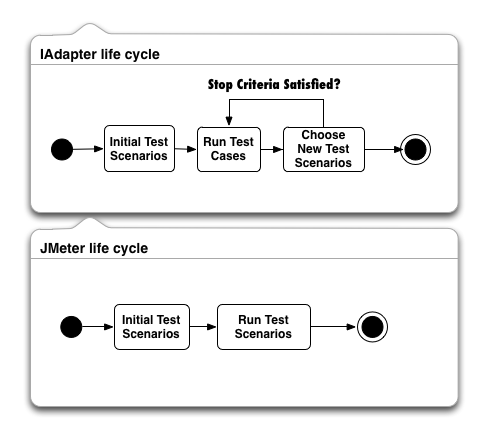
\includegraphics[width=0.5\textwidth]{./images/lifecycle2.png}
\caption{IAdapter life cycle}
\label{fig:iadapterlifecycle}
\end{figure}


The testbed tool proposed consists of four main elements. The first element is a emulator module that it is responsible to simulate the antipatterns in a specific context. The second it's a module named test module that it is responsible for use a previous selected metaheuristics and perform a search based test. The third module contains the test scenarios representation. The fourth module it is responsible for provide a service of explore the neighborhood of a given individual. The Fig. \ref{fig:testbedarch} presents the main architecture of the Testbed solution proposed. The emulator module provides workloads to the Test module.The Test module uses a class loader to find all classes that extends AbstractAlgorithm in the classpath and run all tests for each metaheuristic found. The Test Scenario Representation and Persistent Module provides the scenario representation used by the metaheuristics and persist the testbed results data in a database. Neighborhood provider service is responsible to search neighbors of some individual provided as parameter to the service.

\begin{figure}[H]
\centering
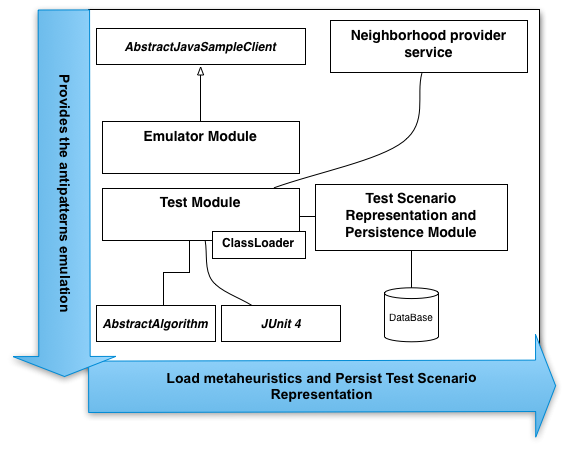
\includegraphics[width=0.6\textwidth]{./images/testbedarch.png}
\caption{testbed main architecture.}
\label{fig:testbedarch}
\end{figure}

\subsection{Test Module}

The Test Module is responsible for load all classes that extends AbstractAlgorithm in the classpath and perform the tests under the application. The Emulator Module provides successful scenarios and antipatterns implementations. The heuristics are executed in order to select the scenarios with failures or high response times. The Fig. \ref{fig:step1} presents the first feature of Test Module where a initial population it is created and IAdapter with JMeterEngine performs all tests and apply a fitnesse value to each workload.

\begin{figure}[H]
\begin{minipage}{.5\textwidth}
\centering
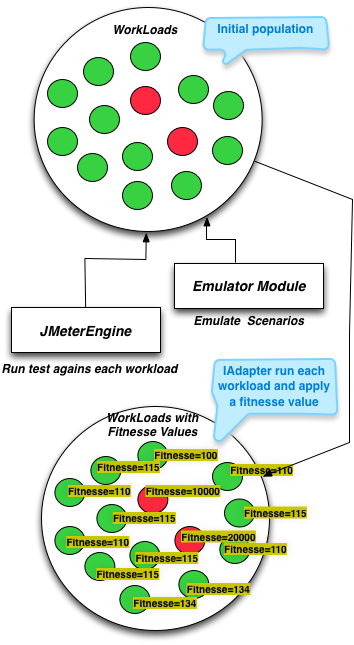
\includegraphics[width=0.8\textwidth]{./images/step1.png}
\caption{Test Module first feature.}
\label{fig:step1}
\end{minipage}
\begin{minipage}{.5\textwidth}
\centering
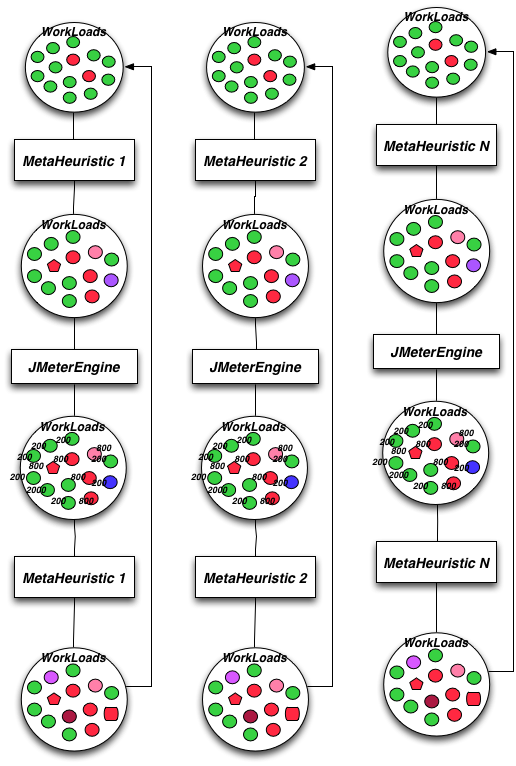
\includegraphics[width=1\textwidth]{./images/step2.png}
\caption{Test Module life cycle.}
\label{fig:step2}
\end{minipage}
\end{figure} 

The Fig. \ref{fig:step2} presents the Test Module life cycle. The life cycle iterate over two steps: The first step apply a metaheurist to select or generate a new set of workloads based on selection criteria. The second step run each workload with the JMeterEngine and obtain a fitnesse value based on some objective function. The red circles represent the workload that contain errors. The green circles represents the workloads with no errors and low acceptable response time. The testbed tool uses as default objective function the equation:


\begin{equation}
\begin{aligned}
fitnesse=90percentileweigth* 90percentiletime\\
+80percentileweigth*80percentiletime\\+
70percentileweigth*70percentiletime+\\
maxResponseWeigth*maxResponseTime+\\
numberOfUsersWeigth*numberOfUsers-penalty
\end{aligned}
\end{equation}

The use of presented fitnesse value by each metaheuristic it's optional. Each Metaheuristic could define your own objective function. The proposed  fitness function uses a series of manually adjustable user-defined weights (90percentileweight, 80percentileweight,  70percentileweight, maxResponseWeight, and numberOfUsersWeight). These weights make it possible to customize the search plugin's functionality. A penalty is applied when an application under test takes a longer time to respond than the level of service. After all these steps the cycle begins until the maximum number of generations it is reached. The Fig. \ref{fig:heuristicclassdiagram} shows the  class diagram for custom and provided heuristics. All heuristic classes extends the class AbstractAlgorithm. The heuristics receives  as input a  list of workspaces and a list of testcases. The workspace represents each individual in the search space.


\begin{figure}[H]
\centering
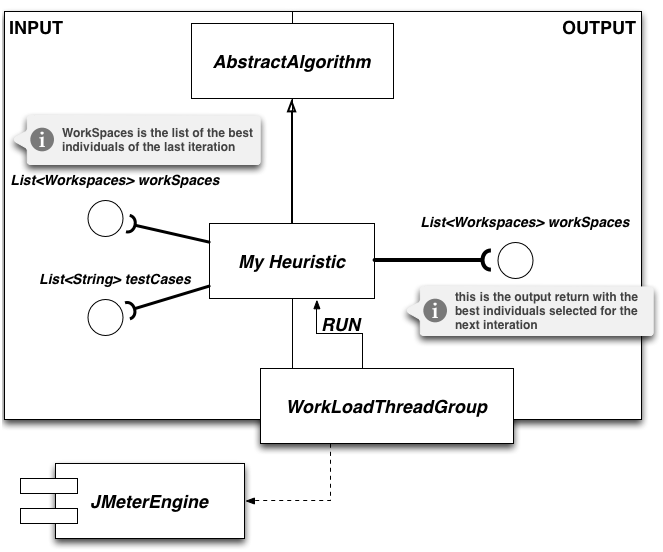
\includegraphics[width=0.6\textwidth]{./images/myheuristic.png}
\caption{Heuristic class diagram.}
\label{fig:heuristicclassdiagram}
\end{figure}  


Each metaheuristic class returns a list of workspaces (the individuals selected to the next generation). The Listing presents the method that performs the search of classes that extends Abstract Algorithm

\begin{lstlisting}[caption={Sample of JDBC emulated by the Mockito Framework}]
public static List<String> getClasses() {

		List<String> list = new ArrayList<String>();

		Reflections reflections = new Reflections("br.unifor.iadapter");
		Set classes = reflections.getSubTypesOf(AbstractAlgorithm.class);
		for (Object object : classes) {
			list.add(((Class) object).getCanonicalName());
		}
		
		return list;
	}
\end{lstlisting}

\subsection{Emulator Module}

The Emulator Module is responsible for implement and provide successful scenarios and the most commons performance antipatterns. All classes must extends the AbstractJavaSamplerClient class or use JUnit 4. The AbstractJavaSamplerClient class allows create a JMeter Java Request.  Using JUnit 4, the emulators classes could be called by a JMeter JUnit request. The Fig. \ref{fig:emulator} presents the main features of the emulator module. The module implements 8 test scenarios in its first version.

\begin{figure}[H]
\centering
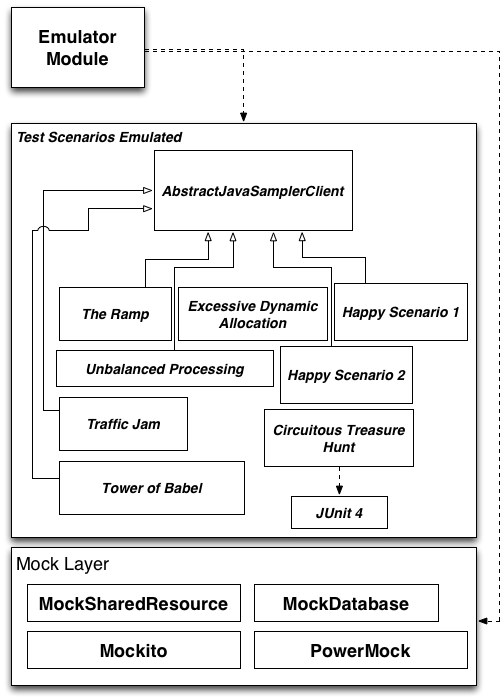
\includegraphics[width=0.6\textwidth]{./images/emulator.png}
\caption{Heuristic class diagram.}
\label{fig:emulator}
\end{figure}  

The Mock Layer provides emulated databases and components to the test scenarios. Each scenario provided by the Emulator Module could be called in JMeter using a Java Request. The algorithm \ref{unbalancedalgorithm} emulates the Unbalanced Processing antipattern. The test scenario C still waiting until A and B scenarios are used by a test.

\begin{algorithm}[H]
  \caption{Unbalanced Processing emulate algorithm}\label{unbalancedalgorithm}
  \begin{algorithmic}[1]
    
    \While{ List of processing scenarios contains A and B }
    \State Processing A and B scenarios
    \EndWhile
    \State Processing scenario C
      
  \end{algorithmic}
\end{algorithm}

The algorithm \ref{rampalgorithm} emulates  the Ramp antipattern. The algorithm increase the response time at each  time that it has been used.

\begin{algorithm}[H]
  \caption{The Ramp emulate algorithm}\label{rampalgorithm}
  \begin{algorithmic}[1]
    \If {count is null}
    \State $count \gets 0  $
    \EndIf
    \State sleep(100* count)
    \State $count \gets count +1  $     
  \end{algorithmic}
\end{algorithm}


The algorithm \ref{excessivedynamicallocation} implements the Excessive Dynamic Allocation antipattern. The algorithm creates a connection with a emulated database, uses the connection and finally the connection.

\begin{algorithm}[H]
  \caption{Excessive Dynamic Allocation emulate algorithm}\label{excessivedynamicallocation}
  \begin{algorithmic}[1]
    
    \For{\textbf{each} request}
        \For{int i=0 to 1000}
        \State Create a connection to a database
        \State Use the connection
        \State Destroy the created connection     
        \EndFor
    \EndFor
      
  \end{algorithmic}
\end{algorithm}

The algorithm \ref{happyscenario1} presents the Happy Scenario 1. The response time increases for every 10 users.

\begin{algorithm}[H]
  \caption{Happy Scenario 1 emulate algorithm}\label{happyscenario1}
  \begin{algorithmic}[1]
    \If {users > 10 and  users<20}
    \State sleep(10*users)
    \EndIf    
    \If {users >= 20 and users<30}
    \State sleep(20*users)
    \EndIf    
    \If {users >= 30 and users<40}
    \State sleep(30*users)
    \EndIf        
    \If {users >= 40 and users<50}
    \State sleep(40*users)
    \EndIf        
    \If {users >= 50 and users<60}
    \State sleep(60*users)
    \EndIf        
    \If {users >= 60 and users<70}
    \State sleep(70*users)
    \EndIf
    \If {users >= 80 and users<90}
    \State sleep(80*users)
    \EndIf      
     \If {users >= 90 }
    \State sleep(90*users)
    \EndIf                  
  \end{algorithmic}
\end{algorithm}

A further 4 algorithms were developed for the scenarios  Circuitous Treasure Hunt, Happy Scenario 2, Traffic Jam and Tower of Babel.

\subsection{Test Scenario Representation Module}

This modules provides a set of scenarios in a common representation. The representation of a scenario is composed by a linear vector with 23 positions. The first position represents the name of an individual. The second position represents the algorithm (genetic algorithm, simulated annealing, or Tabu search) used by the individual. The third position represents the type of test (load, stress, or performance). The next positions represent 10 scenarios and their numbers of users. Each scenario is an atomic operation: the scenario must log into the application, run the task goal, and undo any changes performed, returning the application to its original state.

Fig. \ref{fig:genomarepresentation} presents the solution representation and an example using the crossover operation. In the example, genotype 1 has the Login scenario with 2 users, the Form scenario with 0 users, and the Search scenario with 3 users. Genotype 2 has the Delete scenario with 10 users, the Search scenario with 0 users, and the Include scenario with 5 users. After the crossover operation, we obtain a genotype with the Login scenario with 2 users, the Search scenario with 0 users, and the Include scenario with 5 users.

\begin{figure}[h]
\centering
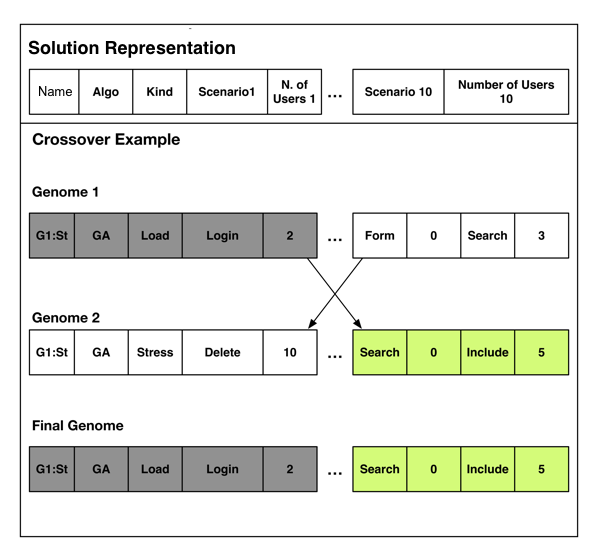
\includegraphics[width=0.5\textwidth]{./images/genomerepresentation1.png}
\caption{Solution representation and crossover example}
\label{fig:genomarepresentation}
\end{figure}


\subsection{Neighborhood provider service}


Fig. \ref{fig:neighbourtaby} shows the strategy used by the proposed solution to obtain the representation of the neighbors for the Tabu search and simulated annealing algorithms. The neighbors are obtained by the modification of a single position (scenario or number of users) in the vector.


\begin{figure}[h]
\centering
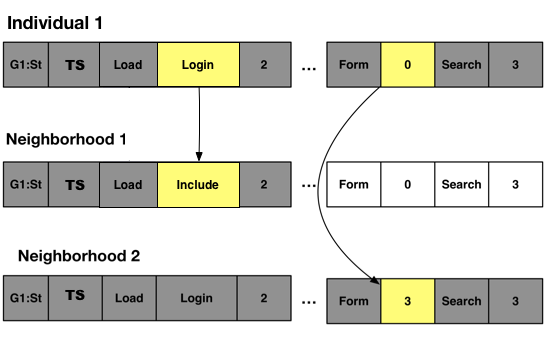
\includegraphics[width=0.4\textwidth]{./images/neighbor.png}
\caption{Neighborhood provider strategy}
\label{fig:neighbourtaby}
\end{figure}

\FloatBarrier
\section{Experiments}

In this section, we conducted experiments in order to verify the effectiveness of the testbed. The first experiment ran for 20 generations, and the second experiment  performed  generations, with . The experiments used an initial population of 100 individuals. The genetic algorithm used the top 10 individuals from each generation in the crossover operation. The Tabu list was configured with the size of 10 individuals and expired every 2 generations.  The mutation operation was applied to 10\% of the population on each generation. 


The experiments used the following fitness (goal) function:

\begin{equation}
\begin{aligned}
fit=90* 90percentiletime\\
+20*80percentiletime\\+
10*70percentiletime+\\
10*maxResponseTime+\\
10*numberOfUsers-penalty
\end{aligned}
\end{equation}

A penalty is applied when the response time is greater than the  maximum response time expected. The penalty is calculated by the follow equation:

\begin{equation}
\begin{aligned}
penalty=100 * \Delta \\
\Delta=(t_{Current Response Time} \\
- t_{Maximum Response Time Expected})\\
\end{aligned}
\end{equation}

This research addresses to verify if the emulated antipatterns could be applied in a testbed. The next subsections present details about the two experiments.


\subsection{The Ramp and Circuitous Treasure Hunt experiment}

This experiment was performed in six 20 generations with three scenarios (The Ramp, Circuitous Treasure Hunt and Happy Scenario 1). The experiment has the following goals:

\begin{itemize}
\item (Goal 1) find the scenarios whose response time has a value of up to 5 seconds. 
\item (Goal 2) Identify and penalize the scenarios that contains the Ramp or Circuitous Treasure Hunt antipattern.
\item (Goal 3) Identify the algorithms with better fitnesse value and response time.
\end{itemize}

The experiment uses tabu search, hill climbing,  genetic algorithms and the hybrid metaheuristic approach proposed by Gois et al. \cite{Gois2016}. Scenarios were generated with the Ramp and Circuitous Treasure antipattern as well as scenarios with Happy Scenario 1 and mixed scenarios. The Fig. \ref{fig:hybridhill} presents the fitnesse value obtained by The Hybrid metaheuristic approach in comparasion with Hill Climbing metaheuristic.   The Fig. \ref{fig:hybridgenetic} presents the comparasion between Hybrid metaheuristic and genetic algorithms. The Fig. \ref{fig:hybridtabu} presents the comparasion between Hybrid metaheuristic and Tabu Search. The Hybrid scenario ussually obtained better fitnesse value than all the others metaheuristics (Goal 3). The higher the fit value, the average response time it is closer to 5 seconds (Fig. \ref{fig:fitresponsetime} ).


\begin{figure}[H]
\begin{minipage}{.5\textwidth}
\centering
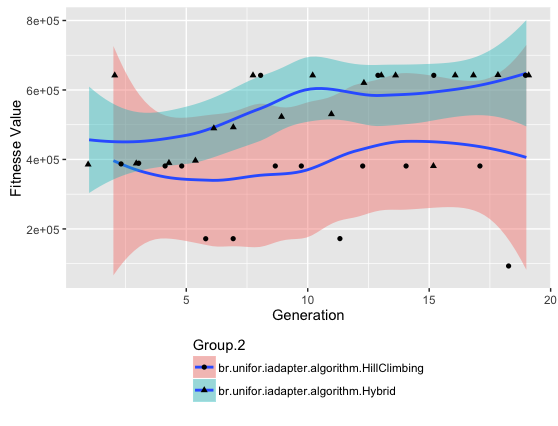
\includegraphics[width=1\textwidth]{./images/experiment-1.png}
\caption{Comparison between Hybrid and Hill Climbing algorithms}
\label{fig:hybridhill}
\end{minipage}
\begin{minipage}{.5\textwidth}
\centering
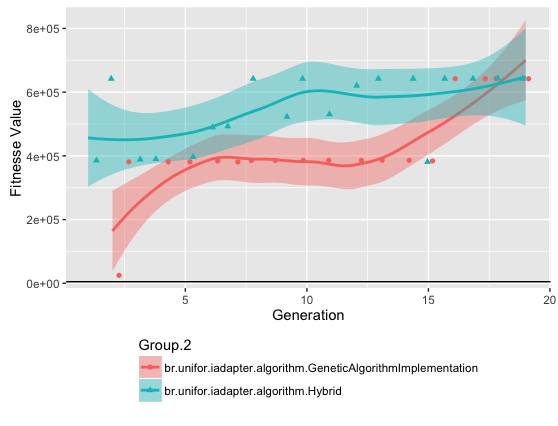
\includegraphics[width=1\textwidth]{./images/experiment-2.png}
\caption{Comparison between Hybrid and Genetic algorithms}
\label{fig:hybridgenetic}
\end{minipage}
\end{figure}


\begin{figure}[H]
\begin{minipage}{.5\textwidth}
\centering
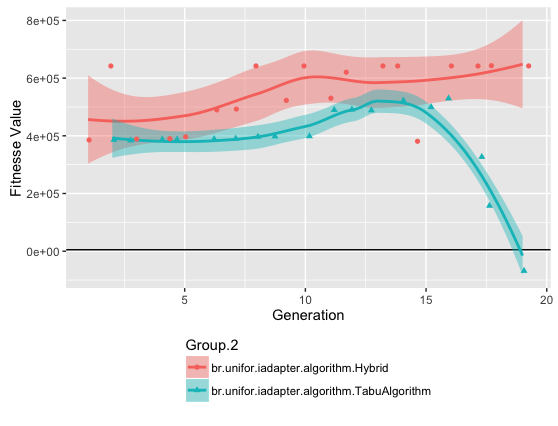
\includegraphics[width=1\textwidth]{./images/experiment-3.png}
\caption{Comparison between Hybrid and Tabu Search algorithms}
\label{fig:hybridtabu}
\end{minipage}
\begin{minipage}{.5\textwidth}
\centering
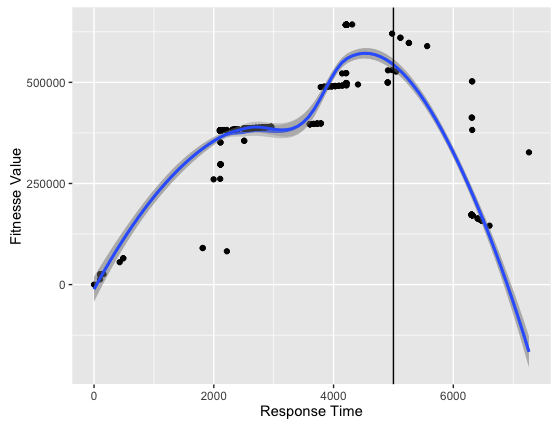
\includegraphics[width=1\textwidth]{./images/experiment-4.png}
\caption{Fitnesse value by response time}
\label{fig:fitresponsetime}
\end{minipage}
\end{figure}

The Fig. \ref{fig:responsetimegeneration} presents the average response time value by generation of the tests that have only  the Happy Scenario 1. The Fig. \ref{fig:fitnessegeneration} presents the fitnesse  value by generation of the tests that have only  the Happy Scenario 1. The response time and fitnesse value is linearly increased over the course of the new generations until tests finds workloads with 5 seconds of response time.

\begin{figure}[H]
\begin{minipage}{.5\textwidth}
\centering
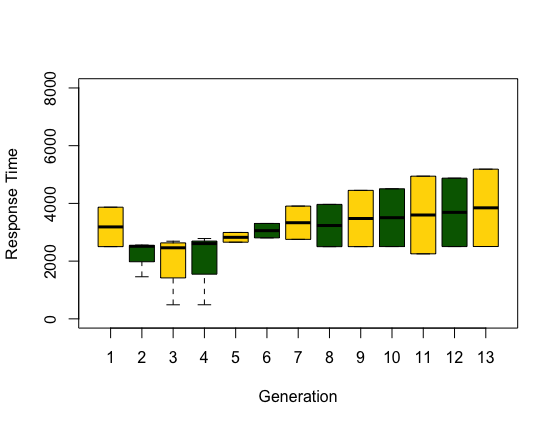
\includegraphics[width=1\textwidth]{./images/experiment-5.png}
\caption{Response time by generation in tests without the Ramp scenario}
\label{fig:responsetimegeneration}
\end{minipage}
\begin{minipage}{.5\textwidth}
\centering
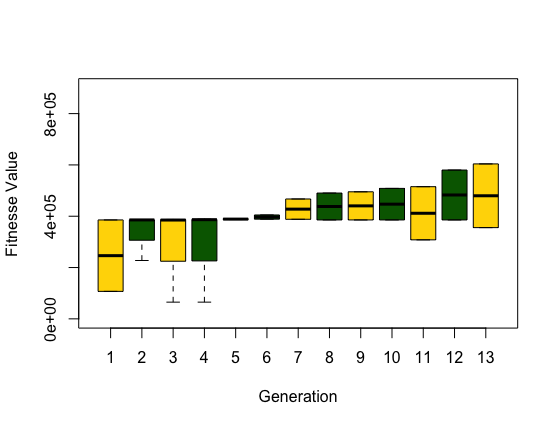
\includegraphics[width=1\textwidth]{./images/experiment-6.png}
\caption{Fitnesse value by generation in tests without the Ramp scenario}
\label{fig:fitnessegeneration}
\end{minipage}
\end{figure}



Table \ref{table:testsexperiment1} shows  9 tests  where the response time of 5 seconds is reached. While the happy scenario reaches the time of 5 seconds with a range of 71 to 75 users (Test 4 to 8), the implementation of the antipattern The Ramp requires only 2 users with 7 to 11 users of the happy scenario.

% Please add the following required packages to your document preamble:
% \usepackage[table,xcdraw]{xcolor}
% If you use beamer only pass "xcolor=table" option, i.e. \documentclass[xcolor=table]{beamer}
\begin{table}[h]
\centering
\caption{9 tests with response time of 5 seconds}
\label{table:testsexperiment1}
\begin{tabular}{l|l|l|l|l|l|l|l|}
\cline{2-8}
 & \cellcolor[HTML]{FFCCC9}\textbf{Users} & \cellcolor[HTML]{FFCCC9}\textbf{Gen} & \cellcolor[HTML]{FFCCC9}\textbf{\begin{tabular}[c]{@{}l@{}}Fit.\\ Value\end{tabular}} & \cellcolor[HTML]{FFCCC9}\textbf{\begin{tabular}[c]{@{}l@{}}Response Time\\ 90\% percentile\end{tabular}} & \cellcolor[HTML]{FFCCC9}\textbf{\begin{tabular}[c]{@{}l@{}}Response Time\\ 80\% percentile\end{tabular}} & \cellcolor[HTML]{FFCCC9}\textbf{\begin{tabular}[c]{@{}l@{}}Response Time\\ 70\% percentile\end{tabular}} & \cellcolor[HTML]{FFCCC9}\textbf{Scenarios} \\ \hline
\multicolumn{1}{|l|}{Test 1} & 9 & 18 & 643200 & 5000 & 5000 & 200 & \begin{tabular}[c]{@{}l@{}}TheRamp (2 Users) and \\ Happy Scn. (7 Users)\end{tabular} \\ \hline
\multicolumn{1}{|l|}{Test 2} & 13 & 18 & 642310 & 5000 & 5000 & 200 & \begin{tabular}[c]{@{}l@{}}TheRamp (2 Users) and \\  Happy Scn. (11 Users)\end{tabular} \\ \hline
\multicolumn{1}{|l|}{Test 3} & 9 & 18 & 642270 & 5000 & 5000 & 5000 & \begin{tabular}[c]{@{}l@{}}TheRamp (2 Users) and\\  Happy Scn. (11 Users)\end{tabular} \\ \hline
\multicolumn{1}{|l|}{Test 4} & 71 & 12 & 620480 & 5000 & 4000 & 3000 & Happy Scenario \\ \hline
\multicolumn{1}{|l|}{Test 5} & 73 & 12 & 610290 & 5000 & 4000 & 3000 & Happy Scenario \\ \hline
\multicolumn{1}{|l|}{Test 6} & 73 & 13 & 610200 & 5000 & 4000 & 3000 & Happy Scenario \\ \hline
\multicolumn{1}{|l|}{Test 7} & 75 & 13 & 597710 & 5000 & 4000 & 3000 & Happy Scenario \\ \hline
\multicolumn{1}{|l|}{Test 8} & 75 & 12 & 597350 & 5000 & 4000 & 3000 & Happy Scenario \\ \hline
\multicolumn{1}{|l|}{Test 9} & 31 & 18 & 589640 & 6000 & 5000 & 5000 & \begin{tabular}[c]{@{}l@{}}Happy Scn. (30 Users) and \\ The Ramp (1 User)\end{tabular} \\ \hline
\end{tabular}
\end{table}


 The Fig. \ref{fig:responsetimegenerationalltests} presents the response time by generation with and without antipatterns scenarios. The Fig. \ref{fig:fitnessegenerationalltests} presents the response time by generation with and without antipatterns scenarios. The red squares are tests with antipattern scenarios. The green squares are tests without the antipattern scenarios. It is possible to observe that the tests with no anti pattern scenarios has response time up to 6 seconds and the scenarios with The Ramp and Circuitous Treasure Hunt antipatterns was penalized with negative values to fitnesse value (Goal 2).


\begin{figure}[H]
\begin{minipage}{.5\textwidth}
\centering
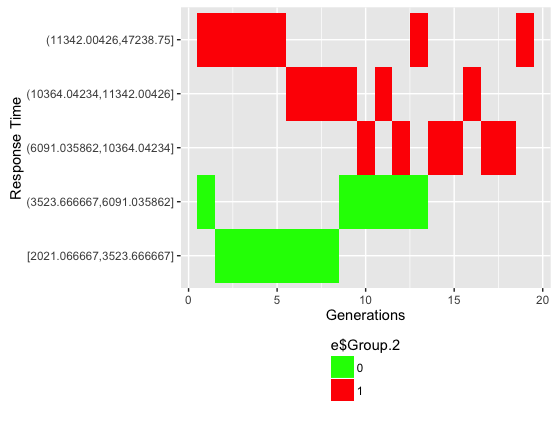
\includegraphics[width=0.8\textwidth]{./images/experiment-7.png}
\caption{Response time by generation in all tests scenarios}
\label{fig:responsetimegenerationalltests}
\end{minipage}
\begin{minipage}{.5\textwidth}
\centering
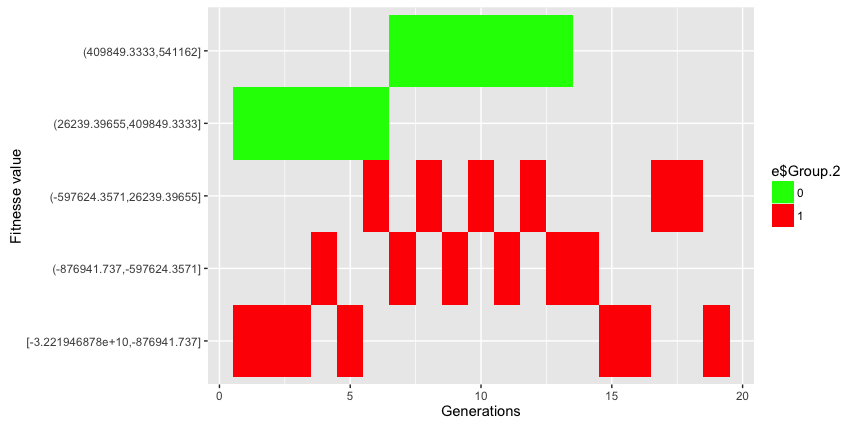
\includegraphics[width=1\textwidth]{./images/experiment-8.png}
\caption{Finesse value by generation in all tests}
\label{fig:fitnessegenerationalltests}
\end{minipage}

\end{figure}

\FloatBarrier
\section{Conclusion}
\FloatBarrier

\bibliography{ecrc-template}
\bibliographystyle{elsarticle-num}

\end{document}

%%
%% End of file `ecrc-template.tex'. 